\documentclass[reqno]{amsart} \usepackage{graphicx, amsmath, amssymb, amsfonts, amsthm, stmaryrd, amscd}
\usepackage[usenames, dvipsnames]{xcolor}
\usepackage{tikz}
% \usepackage{tikzcd}
% \usepackage{comment}

% \let\counterwithout\relax
% \let\counterwithin\relax
% \usepackage{chngcntr}

\usepackage{enumerate}
% \usepackage{enumitem}
% \usepackage{times}
\usepackage[normalem]{ulem}
% \usepackage{minted}
% \usepackage{xypic}
% \usepackage{color}


% \usepackage{silence}
% \WarningFilter{latex}{Label `tocindent-1' multiply defined}
% \WarningFilter{latex}{Label `tocindent0' multiply defined}
% \WarningFilter{latex}{Label `tocindent1' multiply defined}
% \WarningFilter{latex}{Label `tocindent2' multiply defined}
% \WarningFilter{latex}{Label `tocindent3' multiply defined}
\usepackage{hyperref}
% \usepackage{navigator}


% \usepackage{pdfsync}
\usepackage{xparse}


\usepackage[all]{xy}
\usepackage{enumerate}
\usetikzlibrary{matrix,arrows,decorations.pathmorphing}



\makeatletter
\newcommand*{\transpose}{%
  {\mathpalette\@transpose{}}%
}
\newcommand*{\@transpose}[2]{%
  % #1: math style
  % #2: unused
  \raisebox{\depth}{$\m@th#1\intercal$}%
}
\makeatother


\makeatletter
\newcommand*{\da@rightarrow}{\mathchar"0\hexnumber@\symAMSa 4B }
\newcommand*{\da@leftarrow}{\mathchar"0\hexnumber@\symAMSa 4C }
\newcommand*{\xdashrightarrow}[2][]{%
  \mathrel{%
    \mathpalette{\da@xarrow{#1}{#2}{}\da@rightarrow{\,}{}}{}%
  }%
}
\newcommand{\xdashleftarrow}[2][]{%
  \mathrel{%
    \mathpalette{\da@xarrow{#1}{#2}\da@leftarrow{}{}{\,}}{}%
  }%
}
\newcommand*{\da@xarrow}[7]{%
  % #1: below
  % #2: above
  % #3: arrow left
  % #4: arrow right
  % #5: space left 
  % #6: space right
  % #7: math style 
  \sbox0{$\ifx#7\scriptstyle\scriptscriptstyle\else\scriptstyle\fi#5#1#6\m@th$}%
  \sbox2{$\ifx#7\scriptstyle\scriptscriptstyle\else\scriptstyle\fi#5#2#6\m@th$}%
  \sbox4{$#7\dabar@\m@th$}%
  \dimen@=\wd0 %
  \ifdim\wd2 >\dimen@
    \dimen@=\wd2 %   
  \fi
  \count@=2 %
  \def\da@bars{\dabar@\dabar@}%
  \@whiledim\count@\wd4<\dimen@\do{%
    \advance\count@\@ne
    \expandafter\def\expandafter\da@bars\expandafter{%
      \da@bars
      \dabar@ 
    }%
  }%  
  \mathrel{#3}%
  \mathrel{%   
    \mathop{\da@bars}\limits
    \ifx\\#1\\%
    \else
      _{\copy0}%
    \fi
    \ifx\\#2\\%
    \else
      ^{\copy2}%
    \fi
  }%   
  \mathrel{#4}%
}
\makeatother
% \DeclareMathOperator{\rg}{rg}

\usepackage{mathtools}
\DeclarePairedDelimiter{\paren}{(}{)}
\DeclarePairedDelimiter{\abs}{\lvert}{\rvert}
\DeclarePairedDelimiter{\norm}{\lVert}{\rVert}
\DeclarePairedDelimiter{\innerproduct}{\langle}{\rangle}
\newcommand{\Of}[2]{{\operatorname{#1}} {\paren*{#2}}}
\newcommand{\of}[2]{{{{#1}} {\paren*{#2}}}}

\DeclareMathOperator{\Shim}{Shim}
\DeclareMathOperator{\sgn}{sgn}
\DeclareMathOperator{\fdeg}{fdeg}
\DeclareMathOperator{\SL}{SL}
\DeclareMathOperator{\slLie}{\mathfrak{s}\mathfrak{l}}
\DeclareMathOperator{\soLie}{\mathfrak{s}\mathfrak{o}}
\DeclareMathOperator{\spLie}{\mathfrak{s}\mathfrak{p}}
\DeclareMathOperator{\glLie}{\mathfrak{g}\mathfrak{l}}
\newcommand{\pn}[1]{{\color{ForestGreen} \sf PN: [#1]}}
\DeclareMathOperator{\Mp}{Mp}
\DeclareMathOperator{\Mat}{Mat}
\DeclareMathOperator{\GL}{GL}
\DeclareMathOperator{\Gr}{Gr}
\DeclareMathOperator{\GU}{GU}
\def\gl{\mathfrak{g}\mathfrak{l}}
\DeclareMathOperator{\odd}{odd}
\DeclareMathOperator{\even}{even}
\DeclareMathOperator{\GO}{GO}
\DeclareMathOperator{\good}{good}
\DeclareMathOperator{\bad}{bad}
\DeclareMathOperator{\PGO}{PGO}
\DeclareMathOperator{\htt}{ht}
\DeclareMathOperator{\height}{height}
\DeclareMathOperator{\Ass}{Ass}
\DeclareMathOperator{\coheight}{coheight}
\DeclareMathOperator{\GSO}{GSO}
\DeclareMathOperator{\SO}{SO}
\DeclareMathOperator{\so}{\mathfrak{s}\mathfrak{o}}
\DeclareMathOperator{\su}{\mathfrak{s}\mathfrak{u}}
\DeclareMathOperator{\ad}{ad}
% \DeclareMathOperator{\sc}{sc}
\DeclareMathOperator{\Ad}{Ad}
\DeclareMathOperator{\disc}{disc}
\DeclareMathOperator{\inv}{inv}
\DeclareMathOperator{\Pic}{Pic}
\DeclareMathOperator{\uc}{uc}
\DeclareMathOperator{\Cl}{Cl}
\DeclareMathOperator{\Clf}{Clf}
\DeclareMathOperator{\Hom}{Hom}
\DeclareMathOperator{\hol}{hol}
\DeclareMathOperator{\Heis}{Heis}
\DeclareMathOperator{\Haar}{Haar}
\DeclareMathOperator{\h}{h}
\def\sp{\mathfrak{s}\mathfrak{p}}
\DeclareMathOperator{\heis}{\mathfrak{h}\mathfrak{e}\mathfrak{i}\mathfrak{s}}
\DeclareMathOperator{\End}{End}
\DeclareMathOperator{\JL}{JL}
\DeclareMathOperator{\image}{image}
\DeclareMathOperator{\red}{red}
\def\div{\operatorname{div}}
\def\eps{\varepsilon}
\def\cHom{\mathcal{H}\operatorname{om}}
\DeclareMathOperator{\Ops}{Ops}
\DeclareMathOperator{\Symb}{Symb}
\def\boldGL{\mathbf{G}\mathbf{L}}
\def\boldSO{\mathbf{S}\mathbf{O}}
\def\boldU{\mathbf{U}}
\DeclareMathOperator{\hull}{hull}
\DeclareMathOperator{\LL}{LL}
\DeclareMathOperator{\PGL}{PGL}
\DeclareMathOperator{\class}{class}
\DeclareMathOperator{\lcm}{lcm}
\DeclareMathOperator{\spann}{span}
\DeclareMathOperator{\Exp}{Exp}
\DeclareMathOperator{\ext}{ext}
\DeclareMathOperator{\Ext}{Ext}
\DeclareMathOperator{\Tor}{Tor}
\DeclareMathOperator{\et}{et}
\DeclareMathOperator{\tor}{tor}
\DeclareMathOperator{\loc}{loc}
\DeclareMathOperator{\tors}{tors}
\DeclareMathOperator{\pf}{pf}
\DeclareMathOperator{\smooth}{smooth}
\DeclareMathOperator{\prin}{prin}
\DeclareMathOperator{\Kl}{Kl}
\newcommand{\kbar}{\mathchar'26\mkern-9mu k}
\DeclareMathOperator{\der}{der}
% \DeclareMathOperator{\abs}{abs}
\DeclareMathOperator{\Sub}{Sub}
\DeclareMathOperator{\Comp}{Comp}
\DeclareMathOperator{\Err}{Err}
\DeclareMathOperator{\dom}{dom}
\DeclareMathOperator{\radius}{radius}
\DeclareMathOperator{\Fitt}{Fitt}
\DeclareMathOperator{\Sel}{Sel}
\DeclareMathOperator{\rad}{rad}
\DeclareMathOperator{\id}{id}
\DeclareMathOperator{\Center}{Center}
\DeclareMathOperator{\Der}{Der}
\DeclareMathOperator{\U}{U}
% \DeclareMathOperator{\norm}{norm}
\DeclareMathOperator{\trace}{trace}
\DeclareMathOperator{\Equid}{Equid}
\DeclareMathOperator{\Feas}{Feas}
\DeclareMathOperator{\bulk}{bulk}
\DeclareMathOperator{\tail}{tail}
\DeclareMathOperator{\sys}{sys}
\DeclareMathOperator{\atan}{atan}
\DeclareMathOperator{\temp}{temp}
\DeclareMathOperator{\Asai}{Asai}
\DeclareMathOperator{\glob}{glob}
\DeclareMathOperator{\Kuz}{Kuz}
\DeclareMathOperator{\Irr}{Irr}
\newcommand{\rsL}{ \frac{ L^{(R)}(\Pi \times \Sigma, \std, \frac{1}{2})}{L^{(R)}(\Pi \times \Sigma, \Ad, 1)}  }
\DeclareMathOperator{\GSp}{GSp}
\DeclareMathOperator{\PGSp}{PGSp}
\DeclareMathOperator{\BC}{BC}
\DeclareMathOperator{\Ann}{Ann}
\DeclareMathOperator{\Gen}{Gen}
\DeclareMathOperator{\SU}{SU}
\DeclareMathOperator{\PGSU}{PGSU}
% \DeclareMathOperator{\gen}{gen}
\DeclareMathOperator{\PMp}{PMp}
\DeclareMathOperator{\PGMp}{PGMp}
\DeclareMathOperator{\PB}{PB}
\DeclareMathOperator{\ind}{ind}
\DeclareMathOperator{\Jac}{Jac}
\DeclareMathOperator{\jac}{jac}
\DeclareMathOperator{\im}{im}
\DeclareMathOperator{\Aut}{Aut}
\DeclareMathOperator{\Int}{Int}
\DeclareMathOperator{\PSL}{PSL}
\DeclareMathOperator{\co}{co}
\DeclareMathOperator{\irr}{irr}
\DeclareMathOperator{\prim}{prim}
\DeclareMathOperator{\bal}{bal}
\DeclareMathOperator{\baln}{bal}
\DeclareMathOperator{\dist}{dist}
\DeclareMathOperator{\RS}{RS}
\DeclareMathOperator{\Ram}{Ram}
\DeclareMathOperator{\Sob}{Sob}
\DeclareMathOperator{\Sol}{Sol}
\DeclareMathOperator{\soc}{soc}
\DeclareMathOperator{\nt}{nt}
\DeclareMathOperator{\mic}{mic}
\DeclareMathOperator{\Gal}{Gal}
\DeclareMathOperator{\st}{st}
\DeclareMathOperator{\std}{std}
\DeclareMathOperator{\diag}{diag}
\DeclareMathOperator{\Sym}{Sym}
\DeclareMathOperator{\gr}{gr}
\DeclareMathOperator{\aff}{aff}
\DeclareMathOperator{\Dil}{Dil}
\DeclareMathOperator{\Lie}{Lie}
\DeclareMathOperator{\Symp}{Symp}
\DeclareMathOperator{\Stab}{Stab}
\DeclareMathOperator{\St}{St}
\DeclareMathOperator{\stab}{stab}
\DeclareMathOperator{\codim}{codim}
\DeclareMathOperator{\linear}{linear}
\newcommand{\git}{/\!\!/}
\DeclareMathOperator{\geom}{geom}
\DeclareMathOperator{\spec}{spec}
\def\O{\operatorname{O}}
\DeclareMathOperator{\Au}{Aut}
\DeclareMathOperator{\Fix}{Fix}
\DeclareMathOperator{\Opp}{Op}
\DeclareMathOperator{\opp}{op}
\DeclareMathOperator{\Size}{Size}
\DeclareMathOperator{\Save}{Save}
% \DeclareMathOperator{\ker}{ker}
\DeclareMathOperator{\coker}{coker}
\DeclareMathOperator{\sym}{sym}
\DeclareMathOperator{\mean}{mean}
\DeclareMathOperator{\elliptic}{ell}
\DeclareMathOperator{\nilpotent}{nil}
\DeclareMathOperator{\hyperbolic}{hyp}
\DeclareMathOperator{\newvector}{new}
\DeclareMathOperator{\new}{new}
\DeclareMathOperator{\full}{full}
\newcommand{\qr}[2]{\left( \frac{#1}{#2} \right)}
\DeclareMathOperator{\unr}{u}
\DeclareMathOperator{\ram}{ram}
% \DeclareMathOperator{\len}{len}
\DeclareMathOperator{\fin}{fin}
\DeclareMathOperator{\cusp}{cusp}
\DeclareMathOperator{\curv}{curv}
\DeclareMathOperator{\rank}{rank}
\DeclareMathOperator{\rk}{rk}
\DeclareMathOperator{\pr}{pr}
\DeclareMathOperator{\Transform}{Transform}
\DeclareMathOperator{\mult}{mult}
\DeclareMathOperator{\Eis}{Eis}
\DeclareMathOperator{\reg}{reg}
\DeclareMathOperator{\sing}{sing}
\DeclareMathOperator{\alt}{alt}
\DeclareMathOperator{\irreg}{irreg}
\DeclareMathOperator{\sreg}{sreg}
\DeclareMathOperator{\Wd}{Wd}
\DeclareMathOperator{\Weil}{Weil}
\DeclareMathOperator{\Th}{Th}
\DeclareMathOperator{\Sp}{Sp}
\DeclareMathOperator{\Ind}{Ind}
\DeclareMathOperator{\Res}{Res}
\DeclareMathOperator{\ini}{in}
\DeclareMathOperator{\ord}{ord}
\DeclareMathOperator{\osc}{osc}
\DeclareMathOperator{\fluc}{fluc}
\DeclareMathOperator{\size}{size}
\DeclareMathOperator{\ann}{ann}
\DeclareMathOperator{\equ}{eq}
\DeclareMathOperator{\res}{res}
\DeclareMathOperator{\pt}{pt}
\DeclareMathOperator{\src}{source}
\DeclareMathOperator{\Zcl}{Zcl}
\DeclareMathOperator{\Func}{Func}
\DeclareMathOperator{\Map}{Map}
\DeclareMathOperator{\Frac}{Frac}
\DeclareMathOperator{\Frob}{Frob}
\DeclareMathOperator{\ev}{eval}
\DeclareMathOperator{\pv}{pv}
\DeclareMathOperator{\eval}{eval}
\DeclareMathOperator{\Spec}{Spec}
\DeclareMathOperator{\Speh}{Speh}
\DeclareMathOperator{\Spin}{Spin}
\DeclareMathOperator{\GSpin}{GSpin}
\DeclareMathOperator{\Specm}{Specm}
\DeclareMathOperator{\Sphere}{Sphere}
\DeclareMathOperator{\Sqq}{Sq}
\DeclareMathOperator{\Ball}{Ball}
\DeclareMathOperator\Cond{\operatorname{Cond}}
\DeclareMathOperator\proj{\operatorname{proj}}
\DeclareMathOperator\Swan{\operatorname{Swan}}
\DeclareMathOperator{\Proj}{Proj}
\DeclareMathOperator{\bPB}{{\mathbf P}{\mathbf B}}
\DeclareMathOperator{\Projm}{Projm}
\DeclareMathOperator{\Tr}{Tr}
\DeclareMathOperator{\Type}{Type}
\DeclareMathOperator{\Prop}{Prop}
\DeclareMathOperator{\vol}{vol}
\DeclareMathOperator{\covol}{covol}
\DeclareMathOperator{\Rep}{Rep}
\DeclareMathOperator{\Cent}{Cent}
\DeclareMathOperator{\val}{val}
\DeclareMathOperator{\area}{area}
\DeclareMathOperator{\nr}{nr}
\DeclareMathOperator{\CM}{CM}
\DeclareMathOperator{\CH}{CH}
\DeclareMathOperator{\tr}{tr}
\DeclareMathOperator{\characteristic}{char}
\DeclareMathOperator{\supp}{supp}


\theoremstyle{plain} \newtheorem{theorem} {Theorem} \newtheorem{conjecture} [theorem] {Conjecture} \newtheorem{corollary} [theorem] {Corollary} \newtheorem{proposition} [theorem] {Proposition} \newtheorem{fact} [theorem] {Fact}
\theoremstyle{definition} \newtheorem{definition} [theorem] {Definition} \newtheorem{hypothesis} [theorem] {Hypothesis} \newtheorem{assumptions} [theorem] {Assumptions}
\newtheorem{example} [theorem] {Example}
\newtheorem{assertion}[theorem] {Assertion}
\newtheorem{note}[theorem] {Note}
\newtheorem{conclusion}[theorem] {Conclusion}
\newtheorem{claim}            {Claim}
\newtheorem{homework} {Homework}
\newtheorem{exercise} {Exercise}  \newtheorem{question}[theorem] {Question}    \newtheorem{answer} {Answer}  \newtheorem{problem} {Problem}    \newtheorem{remark} [theorem] {Remark}
\newtheorem{notation} [theorem]           {Notation}
\newtheorem{terminology}[theorem]            {Terminology}
\newtheorem{convention}[theorem]            {Convention}
\newtheorem{motivation}[theorem]            {Motivation}


\newtheoremstyle{itplain} % name
{6pt}                    % Space above
{5pt\topsep}                    % Space below
{\itshape}                   % Body font
{}                           % Indent amount
{\itshape}                   % Theorem head font
{.}                          % Punctuation after theorem head
{5pt plus 1pt minus 1pt}                       % Space after theorem head
% {.5em}                       % Space after theorem head
{}  % Theorem head spec (can be left empty, meaning ‘normal’)

% \theoremstyle{mytheoremstyle}


\theoremstyle{itplain} %--default
% \theoremheaderfont{\itshape}
% \newtheorem{lemma}{Lemma}
\newtheorem{lemma}[theorem]{Lemma}
% \newtheorem{lemma}{Lemma}[subsubsection]

\newtheorem*{lemma*}{Lemma}
\newtheorem*{proposition*}{Proposition}
\newtheorem*{definition*}{Definition}
\newtheorem*{example*}{Example}

\newtheorem*{results*}{Results}
\newtheorem{results} [theorem] {Results}


\usepackage[displaymath,textmath,sections,graphics]{preview}
\PreviewEnvironment{align*}
\PreviewEnvironment{multline*}
\PreviewEnvironment{tabular}
\PreviewEnvironment{verbatim}
\PreviewEnvironment{lstlisting}
\PreviewEnvironment*{frame}
\PreviewEnvironment*{alert}
\PreviewEnvironment*{emph}
\PreviewEnvironment*{textbf}



\numberwithin{theorem}{section}
\numberwithin{equation}{section}

\begin{document}

\title{Follow-Up-Workshop to TP \\
  Next Horizon: Workshop on Open Problems in Harmonic \\
  Analysis and Analytic Number Theory}

\begin{abstract}
  Unedited notes from talks at the Hausdorff Research Institute for ``Follow-Up-Workshop to TP Next Horizon: Workshop on Open Problems in Harmonic Analysis and Analytic Number Theory''.  These notes are incomplete, have not been proofread, and should be considered only a crude approximation to what happened in the lectures, filtered through my own misunderstandings and distractions.  Any errors should be assumed to be due to the note-taker.
\end{abstract}

\date{April 28 -- May 2, 2025}

\maketitle

\tableofcontents

\url{https://www.mathematics.uni-bonn.de/him/assets/2025/2025_schedule_next_horizon_update.pdf}

\section{James Maynard, \textnormal{\emph{Large values of Dirichlet polynomials and the zeta function}}}

We will pitch some of our favorite problems coming from analytic number theory that can be phrased in terms of large values of Dirichlet polynomials, which can in turn be thought of purely in terms of harmonic analysis.  (A similar pitch, made over lunch to Guth in January 2020, led to our result on large values of the zeta function.)

Given large real parameters $N \leq T$ and a number $\sigma \in(\tfrac{1}{2}, 1)$ and a $1$-bounded sequence $(a_n)_{n=N}^{2 N}$ of complex numbers, let $W \subseteq[T, 2 T]$ be a set on which the corresponding Dirichlet polynomial has magnitude at least $N^\sigma$, i.e.,
\begin{equation*}
  \left\lvert   \sum_{n = N}^{2 N} a_n n^{i t} \right\rvert = \left\lvert  \sum_{n = N}^{2 N} a_n e^{i t \log n} \right\rvert
  \geq N^\sigma
  \quad
  \text{ for all } t \in W.
\end{equation*}
Note that $\sigma = 1$ means ``as large as possible''.

\begin{question}\label{question:cq1zc10h0l}
  What is the best upper bound for $\lvert W \rvert$ in terms of $N, T, \sigma$.
\end{question}

Hopefully the question is clear.  We're just askign for large values of these sorts of objects.  We're expecting that as you look for larger and larger values, these should occur less and less frequently.  Most of the time we won't care about specific $1$-bounded sequences -- we'll try to work with general ones.

\begin{conjecture}[Montgomery]\label{conjecture:cq1zc1v2ot}
  We have $\lvert W \rvert \leq T^{o(1)} N^{2 - 2 \sigma}$.
\end{conjecture}

\begin{conjecture}[Montgomery] \label{conjecture:cq1zc11ps1}
  $\int_T^{2 T} \left\lvert \sum_{n = N}^{2 N} a_n n^{i t} \right\rvert^k \, d t \leq T^{o(1)} \left( T N^{k/2} + N^k\right)$.
\end{conjecture}
\begin{itemize}
\item Conjecture \ref{conjecture:cq1zc1v2ot} implies Conjecture \ref{conjecture:cq1zc11ps1} which in turn implies the slightly weaker upper bound $\lvert W \rvert \leq T^{2 - 2 \sigma + o(1)}$.
\item Both of these conjectures are hard in general -- we're not expecting anyone to completely solve them.
\item Bourgain showed that Conjecture \ref{conjecture:cq1zc11ps1} implies the Kakeya conjecture.
\item Conjecture \ref{conjecture:cq1zc11ps1} implies the density hypothesis for $\zeta(s)$:
  \begin{equation*}
    \# \left\{ \rho : \zeta(\rho) = 0, \quad \Re(\rho) \geq \sigma, \, \lvert \Im(\rho) \rvert \leq T \right\}
    \leq T^{2 - 2 \sigma + o(1)}.
  \end{equation*}
\item Lindelöf hypothesis $\leftrightarrow \left\lvert \sum_{N}^{2 N} n^{i t} \right\rvert \leq T^{o(1)} N^{1/2}$.
\item Riemann hypothesis $\leftrightarrow \left\lvert \sum_{N}^{2 N}(\Lambda(n) - 1) n^{i t} \right\rvert \leq T^{o(1)} N^{1/2}$.
\end{itemize}

\begin{remark}
  Is more known about Conjecture \ref{conjecture:cq1zc1v2ot} when $a_n = 1$?  Well, in that case, we can focus on the range $N \approx T^{1/2}$, but then outside the case $k \leq 4$, we don't know much more than for a general $1$-bounded sequence,
\end{remark}

The ``trivial bound'' reads
\begin{align*}
  &\int_T^{2 T} \left\lvert \sum a_n n^{i t} \right\rvert^2 \, d t
  \\
  &\leq \int \omega \left( \frac{t}{T} \right)
    \left\lvert \sum_{n = N}^{2 N} a_n n^{i t} \right\rvert^2 \, d t \\
  &= \sum_{n, m} a_n \overline{a_m} \underbrace
    {
    \int \omega(\tfrac{t}{T}) \left( \frac{n}{m} \right)^{i t} \, d t
    }_{
    \approx
    \begin{cases}
      0
      & \text{ if }       \left\lvert \tfrac{n}{m} - 1 \right\rvert \geq \tfrac{c}{T}, \\
      \O(T)
      & \text{ otherwise}
    \end{cases}
    } \\
  &\leq \sum_{n = m \left( 1 + \O(\tfrac{1}{T}) \right)} T
    \leq T N + N^2.
\end{align*}
Note that $\left\lvert \sum a_n \right\rvert^2$ is also a Dirichlet polynomial of length $N^k$, which implies Montgomery's Conjecture \ref{conjecture:cq1zc11ps1} for $k$ an even integer.  More generally, one obtains
\begin{equation*}
  \lvert W \rvert \leq T N^{k(1 - 2 \sigma)} + N^{2 k(1 - \sigma)}
  \quad \text{ for any integer } k.
\end{equation*}
\textbf{Key point}: for many arithmetic applications, one just needs to beat trivial bounds for specific parameters.

\textbf{Challenge 1}: zero density estimates and primes in short intervals.  This was the specific question motivating our work with Guth.  As a consequence of our work, there is a new limiting case
\begin{equation*}
  \sigma = 7/10, \quad N = T^{5/13},
  \quad(a_n)_N^{2 N} = (1).
\end{equation*}
In this case, the trivial bounds come from looking at the \emph{fourth} moment, which gives $T N^{2 - 4 \frac{7}{10}}$.  \textbf{Can you beat this?}  Our work with Guth \emph{does} beat this if $\sigma > 7/10$, but doesn't use the following features:
\begin{itemize}
\item That $a_n = 1$.
\item That $N = T^{5/13}$ is quite small.  We instead square to get a Dirichlet polynomial of length $T^{10/13}$.  It should, in principle, be possible to do better using that this polynomial is a square.
\item We also can improve except when $\left\lvert \{t_1 + t_2 - t_3 - t_4 = \O(1), \, t \in W\} \right\rvert = \frac{\lvert W \rvert}{T}$.
\end{itemize}

\textbf{Challenge 2}: moments of $\zeta(s)$.  We know that $\int_{T}^{2 T} \left\lvert \zeta(\tfrac{1}{2} + i t) \right\rvert^{4} \leq T^{1 + o(1)}$, and expect the same for all moments, but the next interesting result is $\int_T^{2 T} \left\lvert \zeta(\tfrac{1}{2} + i t) \right\rvert^{12} \, d t \leq T^{2 + o(1)}$.  This implies in particular that $\int_T^{2 T} \left\lvert \zeta(\tfrac{1}{2} + i t) \right\rvert^{\kappa} \leq T^{\tfrac{1}{2} + \tfrac{\kappa}{8} + o(1)}$ for $4 \leq \kappa \leq 12$.  This is the best we know for these intermediary exponents.  The critical case is when $N = T^{1/2}$, $\sigma = 3/4$ (which corresponds to the zeta function taking values of size $T^{1/8}$), and you want to beat the trivial bound $T^{1/2}$ coming from the fourth moment, say for $(a_n)_N^{2 N} =(1)$.  (Our work with Guth was designed for $\sigma = 3/4$ but gives nothing in this case.  We're not using that you're squaring a shorter polynomial.)

\textbf{Challenge 3}: progress towards the Lindelöf hypothesis.  Bourgain: $\left\lvert \zeta(\tfrac{1}{2} + i t) \right\rvert \leq T^{13/84 + o(1)}$.  To improve this bound, you typically want to show that
\begin{equation*}
  \left\lvert \sum_{n = N}^{2 N} n^{i t} \right\rvert
  \leq N^{\tfrac{1}{2}} T^{\tfrac{13}{84} + o(1)}
  \quad \text{ for } N \leq T^{\tfrac{1}{2}}.
\end{equation*}
The hardest case again is morally when $N = T^{1/2}$, corresponding (if we have done our arithmetic correctly) to $\sigma = 17/21$.  Want to show in that case that $\lvert W \rvert = 0$ (shoehorning this $L^\infty$ bound into our original question).

\textbf{Challenge 4}: progress on the zero free region.  This is somewhat more speculative.  For the zero-free region, there is a method of Vinogradov--Korobov that gives
\begin{equation*}
  \left\lvert \sum_{n = N}^{2 N} n^{i t} \right\rvert
  \leq N^{1 - \sigma_0}, \quad
  \sigma_0 \simeq \frac{(\log N)^2}{(\log T)^2}.
\end{equation*}
This is what's behind the best-known zero-free region.  In particular, this is nontrivial for $N \geq \exp\bigl((\log T)^{2/3 + o(1)}\bigr)$.  The question is now essentially, how small can we take $N$ to get a nontrivial bound here?  Essentially, nothing nontrivial is known for $N \leq \exp\bigl((\log T)^{2/3}\bigr)$, so the challenge is to prove something nontrivial when $N$ is of that size.

\section{Maksym Radziwill, \textnormal{\emph{Where we get stuck on the 12th moment of the Riemann zeta function}}}

$\zeta(s) = \sum_{n \geq 1}1 / n^s$ for $\Re(s) > 1$, analytic continuation to (e.g.) $\Re(s) > 0$, functional equation:
\begin{equation*}
  \xi(s) := \pi^{- s/2} \Gamma(s/2) \zeta(s) = \xi(1 - s).
\end{equation*}
In view of this, we can think of $\Re(s) = 1/2$ as a  ``boundary set'' for this analytic function: if you understand it there, you understand it everywhere else.  Coincidentally, the Riemann Hypothesis asserts that all non-real zeros are on the line $\Re(s) = 1/2$.

One can use these properties to show that
\begin{equation*}
  \zeta(\tfrac{1}{2} + i t) \approx \sum_{n < t} \frac{1}{n^{1/2 + i t}}
\end{equation*}
inside the critical strip.  Riemann had the idea of turning this into a more efficient formula.  The observation is based on Poisson summation, which gives
\begin{equation*}
  \sum_{n \sim N}
  \frac{1}{n^{1/2 + i t}}
  \approx e^{i t \log t}
  \sum_{n \sim t / N}
  \frac{1}{n^{1/2 - i t}}.
\end{equation*}
There's thus a duality between $N$ and $t /N$.  Thus, writing $\sum_{n < t} = \sum_{n < \sqrt{t}} + \sum_{\sqrt{t} < n < t}$, splitting the sum into dyadic intervals, applying Poisson and recombining, we get
\begin{equation*}
  \sum_{\sqrt{n} < n < t} \frac{1}{n^{1/2 + i t}} \approx e^{i t \log t} \sum_{n < \sqrt{t}} \frac{1}{n^{1/2 - i t}}.
\end{equation*}
The resulting formula
\begin{equation*}
  \zeta(s) = \sum_{n < \sqrt{t}} \frac{1}{n^{1/2 + i t}} + e^{i t \log t}
  \sum_{n < \sqrt{t}} \frac{1}{n^{1/2 - i t}}
\end{equation*}
is computationally more efficient than the previous formula, and we expect it to be theoretically more efficient, too.  (One can actually do better via Diophantine approximation.  Start with the Annals paper of Ghaith--Hiary.)

The Riemann Hypothesis implies the Lindelöf Hypothesis which says that $\zeta(\tfrac{1}{2} + i t) \ll_\eps(1 + \lvert t \rvert)^\eps$ for every $\eps > 0$.  Compare this with the trivial bound that we get from the approximate functional equation $\zeta(\tfrac{1}{2} + i t) \ll(1 + \lvert t \rvert)^{1/4}$, called the convexity bound.  In many cases, it is useful to know that the Lindelöf Hypothesis holds for ``generic points'' $T \leq t \leq 2 T$.  This is quantified by moments $\int_T^{2 T} \lvert \zeta(\tfrac{1}{2} + i t) \rvert^{2 k} \, d t$.  Since $\zeta$ can be approximated by a Dirichlet polynomial containing the constant term $1$, we have $\int_T^{2 T} \lvert \zeta(\tfrac{1}{2} + i t) \rvert^{2 k} \, d t \gg T$.  On the other hand, the Lindelöf Hypothesis implies that $\int_T^{2 T} \lvert \zeta(\tfrac{1}{2} + i t) \rvert^{2 k} \, d t \ll_\eps T^{1 + \eps}$.  It is htus conjectured that for all $k > 0$, we have
\begin{equation}\label{eq:cq1zddl298}
  \int_T^{2 T} \left\lvert \zeta(\tfrac{1}{2} + i t) \right\rvert^{2 k} \, d t = T^{1 + o(1)}.
\end{equation}
Since for any $T \leq t \leq 2 T$,
\begin{equation}\label{eq:cq1zdd63vg}
  \frac{1}{\log T} \left\lvert \zeta(\tfrac{1}{2} + i t) \right\rvert^{2 k} \ll \int_T^{2 T} \left\lvert \zeta(\tfrac{1}{2} + i t) \right\rvert^{2 k} \, d t,
\end{equation}
we see that the conjecture for moments implies the Lindelöf Hypothesis.  They are thus equivalent.  This was the original idea for introducing moments: embed $\zeta$ in some family of harmonics, which should make things easier to understand.

What do we know about moments?  We get stuck very quickly.  The conjecture \eqref{eq:cq1zddl298} is known only for $k \leq 2$.  To see this, we use the approximation functional equation and plug it into the moment, giving something like
\begin{equation*}
  \int_{T}^{2 T} \left\lvert \zeta(\tfrac{1}{2} + i t) \right\rvert^{2 k} \, d t
  \ll \int_T^{2 T}
  \left\lvert \sum_{n \leq \sqrt{T}} \frac{1}{n^{1/2 + i t}} \right\rvert^{2 k} \, d t.
\end{equation*}
Pulling the $k$th power inside, we get $\int_{T}^{2 T} \left\lvert \left( \sum_{n \leq \sqrt{T}} \frac{1}{n^{1/2 + i t}} \right)^k \right\rvert^2 \, d t$.  This can be rewritten $\int_T^{2 T} \left\lvert \sum_{n \leq T^{k/2}} \frac{c(n)}{n^{1/2 + i t}} \right\rvert^2 \, d t$ for some coefficients $c(n) \ll_\eps n^\eps$.  At this point, we introduce a smooth kernel $1 \leq \Phi(\tfrac{t}{T})$, for $0 \leq t \leq T$, say with the property that $\hat{\Phi}$ is compactly-supported.  Thus we have to compute
\begin{equation*}
  \int_{\mathbb{R}} \left\lvert
    \sum_{n \leq T^{k/2}}
    \frac{c(n)}{ n^{1/2 + i t + i T}}\right\rvert^2
  \Phi \left( \frac{t}{T} \right) \, d t.
\end{equation*}
(Notice the shift $n^{i T}$.)  Opening the square and integrating over $T$ gives
\begin{equation*}
  T \sum_{n, m \leq T^{k/2}}
  \frac{c(n) \overline{c(m)}}{\sqrt{n m}}
  \left( \frac{n}{m} \right)^{i T}
  \hat{\Phi} \left( T \log \frac{n}{m} \right).
\end{equation*}
Since $\hat{\Phi}$ is compactly supported, the sum is restricted to values of $n$ and $m$ such that $\left\lvert \log n/m \right\rvert \leq 1/T$.  These are two types of terms to consider: $n = m$, which we call the diagonal, and $n = m + h$ with $0 < \lvert h \rvert < m/T$, which we call the off-diagonal.

The contribution of the diagonal is $T \sum_{m \leq T^{k/2}} \frac{\lvert c(m) \rvert^2}{m} \ll_\eps T^{1 + \eps}$, and is therefore OK.  If $T^{k/2} < T$, then the off-diagonal does not exist.  And if $T^{k/2} > T$, then the off-diagonal is approximately
\begin{equation*}
  \sum_{M = 2^{\ell} \leq T^{k/2}}
  \frac{1}{ M /T}
  \sum_{h \sim M/T}
  \sum_{m \sim M}
  c(m) \overline{c(m + h)}
  \left( 1 + \frac{h}{m} \right)^{i T}.
\end{equation*}
(Even having an optimal bound for the shifted convolution problem would only solve the moment problem up to the $8$th -- to go beyond that, one would need further cancellation in the sum over $h$.)

When $T^{k/2} < T$, that is $k \leq 2$, there are no off-diagonal terms.  This gives the conjecture in such cases.  Those are still the only cases in which we know the correct exponent in the moment conjecture.  Dealing with off-diagonal terms is hard, though not impossible.  Heath--Brown's $12$th moment bound:
\begin{equation*}
  \int_{T}^{2 T} \left\lvert \zeta(\tfrac{1}{2} + i t) \right\rvert^{2 t} \, d t \ll T^2.
\end{equation*}
Using \eqref{eq:cq1zdd63vg}, we deduce then that $\zeta(\tfrac{1}{2} + i t) \ll(1 + \lvert t \rvert)^{1/6 + o(1)}$.  Using Holder's inequality, we get
\begin{equation*}
  \int_{T}^{2 T} \left\lvert \zeta(\tfrac{1}{2} + i t) \right\rvert^{2 k} \, d t \ll T^{1 +(2 k - 4) / 8}.
\end{equation*}
Those are the best results currently known for all moments with $k \leq 6$.  There are results for higher $k$ generalizing Heath--Brown's result, but they are of little interest, and interpolation against them leads to weaker exponents for $k \leq 6$.  I will explain shortly why they are of little interest.  The distribution content of Heath--Brown's result is that
\begin{equation*}
  \vol \{\lvert \zeta(\tfrac{1}{2} + i t) \rvert > V\} \ll \frac{1}{V^{12}} \int_T^{2 T} \left\lvert \zeta(\tfrac{1}{2} + it) \right\rvert^{12} \, d t
  \ll \frac{T^2}{V^{12}}.
\end{equation*}
Compare it with the $4$th moment, that gives
\begin{equation*}
  \frac{1}{V^4} \int_T^{2 T}
  \left\lvert \zeta(\tfrac{1}{2} + i t) \right\rvert^4 \, d t
  \ll \frac{T^{1 + o(1)}}{V^4}.
\end{equation*}
This means that Heath--Brown's result is stronger than the fourth moment for $V > T^{1/8}$ and weaker for $V < T^{1/8}$.

Thus the key point to improve on Heath--Brown's result is to show that $\vol\{ \lvert \zeta(\tfrac{1}{2} + i t) \rvert > T^{1/8} \} \ll T^{1/2 - \delta}$ for some $\delta > 0$.  This would improve the exponent in al moments with $4 < 2 k < 12$.  Improving the exponent in the eighth moment would have application to understand the variance of partial sums of $d_4(n)$, for instance.

What is the meaning of this level set?  If we use the approximate functional equation, we need to understand when
\begin{equation*}
  \left\lvert \sum_{n < \sqrt{T}} \frac{1}{ n^{1/2 + i t}} \right\rvert > T^{1/8}.
\end{equation*}
Imagine that this localized at $n \sim \sqrt{T}$ and $n^{1/2} \sim T^{1/4}$.  We then need to understand the level set
\begin{equation*}
  \left\lvert \sum_{n \sim \sqrt{T}} n^{i t} \right\rvert > T^{3/8}.
\end{equation*}
This means that we have a Dirichlet polynomial of length $N$ and we need to understand the frequency of values that are larger than $N^{3/4}$.  (This is the same range that causes trouble in the Huxley--Ingham bound, so maybe the result of Guth--Maynard is applicable?  Unfortunately, it does not improve, because even Montgomery's conjecture isn't sufficient -- one needs to use something more about the $a_n$.)

Perhaps looking at the value distribution is the wrong move here.  Let's try an attack through coefficients.  To make things simple, let's ofcus on the lowest moment that we can.  The twelfth moment implies $\int_{T}^{2 T} \left\lvert \zeta(\tfrac{1}{2} + i t) \right\rvert^6 \, d t \ll T^{5/4}$.  Let's try to understand what it means in terms of coefficients.  It is customary to think of $\zeta(s)^3$ as a $\GL_3$ $L$-function corresponding to an Eisenstein series.  Thus the sixth moment of $\zeta(s)$ is the same thing as the second moment of $\zeta(s)^3$.  This should be similar to the second moment of a general $\GL_3$ $L$-function, say $L(s, \pi)$.  The advantage of looking at this variant is that the coefficients $\lambda_\pi(n)$ of a $\GL_3$ $L$-function are oscillatory,
\begin{equation*}
  L(s, \pi) := \sum_{n \geq 1} \frac{\lambda_\pi(n)}{n^s}.
\end{equation*}
Thus we can think of $\lambda_\pi(n)$ as a variant of $d_3(n)$ but with the ``main term'' taken out.  Let's look, then, at
\begin{equation*}
  \int_{T}^{2 T} \left\lvert L(\tfrac{1}{2} + i t, \pi) \right\rvert^2 \, d t.
\end{equation*}
Applying the approximate functional equation
\begin{equation*}
  \left\lvert L(\tfrac{1}{2} + i t, \pi) \right\rvert \ll \left\lvert \sum_{n \leq T^{3/2}} \frac{\lambda(n)}{n^{1/2 + i t}} \right\rvert
\end{equation*}
and opening the square, a piece of the off-diagonal terms looks like
\begin{equation*}
  \frac{1}{T^{1/2}} \sum_{h \sim T^{1/2}} \sum_{n \sim T^{3/2}} \lambda_\pi(n) \overline{\lambda_\pi(n + h)}.
\end{equation*}
At this stage a reasonable move is to move the sum over $h$ inside and apply Cauchy--Schawrz, giving
\begin{equation*}
  \ll \frac{1}{T^{1/2}} \left( \sum_{n \sim T^{3/2}} \left\lvert \lambda(n) \right\rvert^2 \right)^{1/2}
  \left( \sum_{n \sim T^{3/2}} \left\lvert \sum_{h \sim T^{1/2}} \lambda(n + h) \right\rvert^2 \right)^{1/2}.
\end{equation*}
The best case scenario here is $\sum_{h \sim T^{1/2}} \lambda(n + h) \ll T^{1/4}$, which then just recovers Heath--Brown.

In other words, getting square-root cancellation on average in most short sums over $\lambda(n)$ would only recover Heath--Brown's result.  Thus, to go beyond $T^{5/4}$ it seems that we need to know genuine cancellation in $\sum_{n \sim T^{3/2}} \lambda(n) \overline{\lambda(n + h)}$.  Currently we do not know the existence of a single explicit $h$ such that $\sum_{n \sim N} \lambda(n) \overline{\lambda(n + h)} \ll N^{1 - \delta}$, and correspondingly no asymptotics for $d_3(n)$.  Heath--Brown's bound of $T^{5/4}$ is consistent with this.  We can have $\sum_{n \sim T^{3/2}} \lambda(n) \lambda(n + h) = \eps_\pi T^{3/4}$.

Thus to go beyond in this approach we need not only square root cancellation in the signs $\eps_h$, but also genuine cancellation in $\sum_{n \asymp T^{3/2}} \lambda(n) \lambda(n + h)$ for most $h$.  Part of me is afraid that we won't make progress on the twelfth moment until we manage to show $\sum_{n \leq N} \lambda(n) \lambda(n + h) \ll N^{1 - \delta}$.

Incidentally, the problem of computing the second moment of $L(\tfrac{1}{2} + i t, \pi)$ is genuinely harder than the second moment problem for $\zeta(s)^3$.  Only recently was it shown that
\begin{equation*}
  \int_{T}^{2 T} \left\lvert L(\tfrac{1}{2} + i t, \pi) \right\rvert^2 \, d t \ll T^{3/2 - \delta}
\end{equation*}
for some $\delta > 0$.

Heath--Brown's original approach is based on finding a formula for $\int_t^{t + H} \left\lvert \zeta(\tfrac{1}{2} + i u) \right\rvert^2 \, d u$ and then averaging over $t$ using Halasz--Montgomery.  Iwaniec developed an approach based on finding a formula for $\int_t^{t + H} \left\lvert \zeta(\tfrac{1}{2} + i u) \right\rvert^4 \, d u$ and then averaging over $t$.  Iwaniec's formula is obtained by using the approximate functional equation, and using Kuznetsov's trace formula on the off-diagonal terms (``Kloostermania'').  This leads to a formula roughly of the shape
\begin{equation*}
  \int_{T}^{T + T^{2/3}}
  \left\lvert \zeta(\tfrac{1}{2} + i t) \right\rvert^4 \, d t
  \approx \sum_{t_j} e^{i t_j \log t_j} A_j(\tfrac{1}{2} + i t) B_j(\tfrac{1}{2} + i t),
\end{equation*}
where $\tfrac{1}{4} + t_j^2$ are eigenvalues of the hyperbolic Laplacian,
\begin{equation*}
  A_j(s) := \sum_{n \sim M} \frac{\lambda_j(n)}{n^s},
\end{equation*}
and $\lambda_j(n)$ is the $n$th Fourier coefficient of the automorphic form with eigenvalue $\tfrac{1}{4} + t_j^2$.  Iwaniec then obtains an optimal bound for the above by taking absolute values and ignoring cancellations coming from $e^{i t_j \log t_j}$.  This approach gives $\zeta(\tfrac{1}{2} + i t) \ll(1 + \lvert t \rvert)^{1/6}$.

Recently a sub-Weyl bound of the form
\begin{equation*}
  L(\tfrac{1}{2} + i t, \pi) \ll(1 + \lvert t \rvert)^{1/6 - \delta}
\end{equation*}
was claimed by Holowinsky--Munshi--Sharma--Streipel.

If correct, this might provide an opening for an improvement to Iwaniec's bound and eventually the $12$th moments.  The methods do not appear spectral in nature, but rather close to Bombieri--Iwaniec.

Despite quite a bit of work, the best we can offer a bound of the form
\begin{equation*}
  \int_{T}^{2 T} \left\lvert \zeta(\tfrac{1}{2} + i t) \right\rvert^{2 k} \, d t
  = o \left( T^{1 +(2 k - 4)/8} \right).
\end{equation*}
Maybe saving a small power of a logarithm.  This gives a tiny improvement on Heath--Brown.  This might be enough for the consequence for the variance of $\sum_{n \leq x} d_4(n)$.

What has not worked?
\begin{itemize}
\item Spectral theory and/or Munshi's method
\item Circle method followed by Kuznetsov, which gives tautologies of the kind $A = A + o(1)$, where $A$ on the LHS is the moment and $A$ on the RHS is the same moment appearing as part of the Eisenstein spectrum.
\end{itemize}

The behavior of the $2k$th moment of $\zeta$ is generally speaking tied with the Diophantine properties of $n^{1/k}$.  For example, with de Faveri, we had an alternative proof of Heath--Brown's result using the double large sieve and the result of Robert--Sargos, giving an optimal bound for the number of quadruples $(n_1, n_2, n_3, n_4)$, all of size $N$, such that
\begin{equation*}
  \left\lvert \sqrt{\tfrac{n_1}{N}} + \sqrt{\tfrac{n_2}{N}} - \sqrt{\tfrac{n_3}{N}} - \sqrt{\tfrac{n_4}{N}} \right\rvert \leq \frac{1}{X}.
\end{equation*}
The optimal bound is $\ll N^{\eps} \left( \frac{N^4}{X} + N^2 \right)$.  The proof uses an iterative method, induction on scales, bounding the next thing by the previous thing, so it doesn't give an asymptotic.

If one could refine the result of Robert--Sargos to an asymptotic with a power-saving, there is probably an opening for improving the twelfth moment.

We need this for all of $X$, but really $X$ of size $N^2$ is the main range.

In general, any strong result (i.e., uniform in $X$) on the number of tuples such that
\begin{equation*}
  \left\lvert  \left( \frac{n_1}{N} \right)^{1/k} + \dotsb -  \left( \frac{n_{2 \ell}}{N} \right)^{1/k} \right\rvert \leq \frac{1}{X}
\end{equation*}
can probably be used to improve the $12$th moment.  But I do not believe such results (with $\ell > 2$) are within reach of the current technology.  I am more agnostic on the asymptotic for Robert--Sargos, but the proof of such a result would have to be completely different from the proof of Robert--Sargos (a form of induction on scales).  A radically different idea would be required there.

The new result on sub-Weyl subconvexity for $\GL_2$ $L$-functions might offer ideas on the way forward.

\section{Dominique Maldague, \textnormal{\emph{Difficulty of using decoupling ideas for generalized Dirichlet series and cubic Weyl sums}}}

We'll discuss limitations of decoupling techniques applied to cubic Weyl sums.

Fourier striction theory: control the behavior of functions $f(x)$ (usually in $L^p$-norm) based on properties of the Fourier (or frequency) support, emphasizing geometric properties.

Both examples are going to have inputs $x \in \mathbb{R}^2$.  We'll use the notation $e(\bullet) = e^{2 \pi i(\bullet)}$.

\begin{example}
  $f(x) = \sum_{n = 1}^N e(x \cdot(n, 0))$.  We have $f(0) = N$, $\lvert f(x) \rvert \sim N$ if $\lvert x_1 \rvert < \frac{1}{100 N}$.  We have
  \begin{equation*}
    \int_{[0, 1]^2} \lvert f(x) \rvert^2 \, d x
    =
    \sum_{n, m} \int_{[0, 1]^2}
    e \left( x \cdot(n - m, 0) \right) \, d x = N.
  \end{equation*}

\end{example}


\begin{example}
  $g(x) = \sum_{n = 1}^{N} e(x \cdot(n, n^2))$.  We have $g(0) = N$, $\lvert g(x) \rvert \sim N$ if $\lvert x_1 \rvert < \frac{1}{100 N}$ and $\lvert x_2 \rvert < \frac{1}{100 N^2}$.  We have
  \begin{equation*}
    \int_{[0, 1]^2} \lvert g(x) \rvert^2 \, d x = N.
  \end{equation*}
\end{example}

The first has frequency support consisting of integers in a line.  The second has points on a parabola.  We can also draw pictures indicating where the functions $f$ and $g$ are purely constructively intersecting.  We get a smaller region for $g$ than for $f$: same width, but cut off the height.  It's a bit trickier to describe their intermediate behavior, but we can at least say that they have the same $L^2$ average.

\begin{figure}
  \centering
  \includegraphics[width=0.7\textwidth,angle=-90]{images/img_20250428_145247}
\end{figure}
Let's now consider $p \geq 2$, and ask: how large are the $L^p$-norms?
\begin{equation*}
  N^{p - 1} + N^{p/2} \leq \int_{[0, 1]^2} \lvert f(x) \rvert^p \, d x \leq N^{p - 2} \int \lvert f(x) \rvert^2 \, d x = N^{p - 1}.
\end{equation*}
\begin{equation*}
  N^{p} N^{- \beta} + N^{p/2} \leq \int_{[0, 1]^2}
  \lvert g(x) \rvert^p \, d x.
\end{equation*}
In this last estimate, $N^{p/2}$ dominates for $2 \leq p \leq 6$, and in the same way, we have the same upper bound
\begin{equation}\label{eq:cq1zdx90f3}
  \int_{[0, 1]^2}
  \lvert g(x) \rvert^p \, d x \lessapprox N^{p/2}.
\end{equation}
This type of inequality, where you have square root cancellation behavior for higher $p$: This is an exactly of what you call ``$L^p$-decoupling''.  Easy to check that this is true:
\begin{proof}[Proof of \eqref{eq:cq1zdx90f3}]
  We have
  \begin{equation*}
    \int_{[0, 1]^2} \lvert g(x) \rvert^6 \, d x
    = \sum_{n_1, \dotsc, n_6}
    \lvert g(x) \rvert^6 \, d x
    = \sum_{(n_1, \dotsc, n_6)}
    \int e \left( x \cdot \phi(n) \right) \, d x,
  \end{equation*}
  where
  \begin{equation*}
    \phi(n) =
    (
    n_1 + n_2 + n_3 - n_4 - n_5 - n_6,
    n_1^2 + n_2^2 + n_3^2 - n_4^2 - n_5^2 - n_6^2
    ).
  \end{equation*}
  The integral detects the condition $\phi(n) = 0$.  We obtain the bound $\lessapprox N^3$ by unique factorization.
\end{proof}

What is the continuum picture?  In the continuum setup, we have
\begin{equation*}
  \mathcal{N}_{R^{-1}} \left\{  (\xi, \varphi(\xi)) : \lvert \xi \rvert < 1 \right\}
  =
  \sqcup \Theta,
\end{equation*}
where each $\Theta$ is an $R^{-1/2} \times R^{-1}$ rectangle.  Here $\varphi '' \sim 1$ and $\Phi ' \lesssim 1$.  We consider $f = \sum_{\Theta } f_\Theta$, where each $\supp \hat{f}_\Theta \subseteq \Theta$.  Bourgain--Demeter '16: for $2 \leq p \leq 6$,
\begin{equation*}
  \int_{B_R} \lvert f \rvert^p \lessapprox \left( \sum_{\Theta}
    \left( \int_{B_R} \lvert f_\Theta \rvert^p \right)^{2/p}\right)^{p/12}.
\end{equation*}
From the model case:
\begin{equation*}
  \int_{[0, 1]^2}
  \left\lvert \sum e(x \cdot(n, n^2)) \right\rvert^p \, d x
  \lessapprox N^{p/12}.
\end{equation*}
The left hand side of the above is
\begin{equation*}
  \frac{1}{N^{3+1}} \int_{[0, N] \times[0, N^2]}
  \left\lvert
    \sum e \left( x \cdot \left( \frac{n}{N}, \frac{n^2}{N^2} \right) \right)\right\rvert^p \, d x.
\end{equation*}
We see that $R = N^2$, $f_\Theta(x) = e \left( x \cdot \left( \frac{n}{N}, \frac{n^2}{N^2} \right) \right)$.  The frequency points $(\tfrac{n}{N}, \tfrac{n^2}{N^2})$ are $1/N$-separated.

\begin{figure}
  \centering
  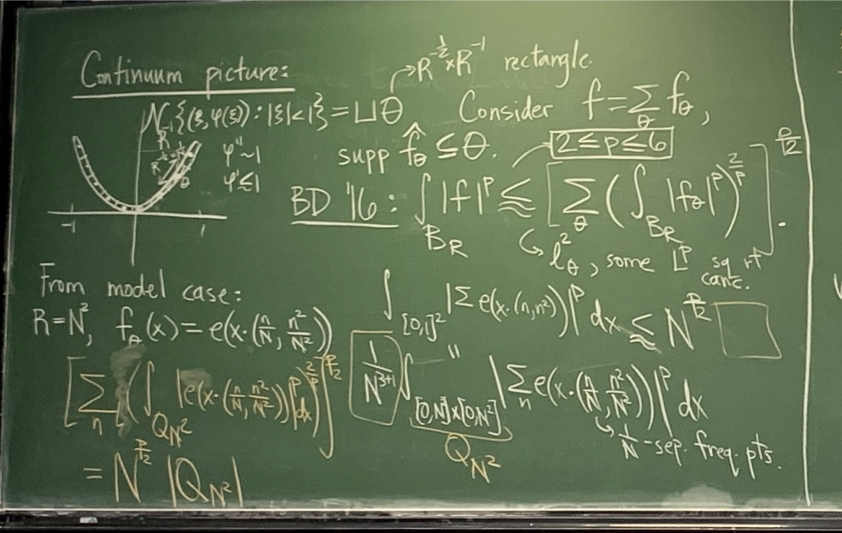
\includegraphics[width=0.9\textwidth]{images/img_20250428_151924}
\end{figure}

Writing $Q_{N^2} :=[0, N] \times[0, N^2]$, we have
\begin{equation*}
  \left[ \sum_n \left( \int_{Q_{N^2}} \left\lvert e\left(x \cdot \left( \frac{n}{N}, \frac{n^2}{N^2} \right)\right) \right\rvert^p \, d x \right)^{2/p} \right]^{p/2}
  = N^{p/2} \left\lvert Q_{N^2} \right\rvert.
\end{equation*}
Bourgain--Demeter decoupling gives
\begin{equation*}
  \int_{Q_{N^2}} \left\lvert \sum_{\xi \in \Lambda}
    e \left( x \cdot(\xi, \varphi(\xi)) \right)\right\rvert^p \, d x
  \lesssim N^{p/2} \left\lvert Q_{N^2} \right\rvert
\end{equation*}
for $2 \leq p \leq 6$, $\Lambda \subseteq[-1, 1]$, $\geq \tfrac{1}{N}$-separated.
\begin{itemize}
\item Sharp (as an inequality) and in the range of $p \in[2, 6]$.
\item Very general.
\item Small cap decoupling (Demeter--Guth--Wang), level set estimates (FGM), amplitude dependent wave envelope estimates (Guth--Maldaque).
\end{itemize}

Which exponential sum problems is decoupling useful for?

\begin{conjecture}
  $\int \left\lvert \sum_{n \sim N} b_n e(t \log n) \right\rvert^p \, d t \lessapprox \left( T N^{p/2} + N  \right) \lVert b_n \rVert_\infty^p$.
\end{conjecture}
The two terms on the right hand side come from square root cancellation and constant interval behavior, respectively.

The frequencies are $\{\log n\}$.  This is a concave sequence: the terms are getting closer and closer to one another.  What happens when you try to apply decoupling is that you don't really get anywhere.  The reason is essentially that the tools of decoupling (wave packets, transversality, locally constant property) apply too generally: they apply to any concave or convex sequence, and some of these sequences have surprising structural properties (e.g., long arithmetic progression subsequences).

There's a related problem: additive energy for convex sequences.
\begin{conjecture}
  $\int_{[0, N^2]} \left\lvert \sum_{n \sim N} e(T a_n)\right\rvert^4  \lessapprox N^4$.
\end{conjecture}
$(a_n)$ has minimal additive energy.  Best bounds not from decoupling!

How about a $2$D question?  We saw
\begin{equation*}
  \int_{Q_{N^2}}
  \left\lvert
    \sum_{\xi \in \Lambda}
    e(x \cdot(\xi, \varphi(\xi)))
  \right\rvert^p
  \,d x
  \lessapprox N^{p/2} \lvert Q_{N^2} \rvert
\end{equation*}
for $2 \leq p \leq 6$.  What happens when we change the size of $Q_{N^2}$?
Shrinking $\rightsquigarrow$ small cap decoupling regime.  Expanding $\rightsquigarrow$ replace $Q_{N^2}$ by $Q_{N^3}$.  We have
\begin{align}
  \int_{Q_{N^3}} \lvert h(x) \rvert^p \, d x
  &= \sum_{Q_{N^2} \subseteq Q_{N^3}}\int_{Q_{N^2}} \left\lvert h(x) \right\rvert^p \, d x
    \lessapprox \sum_{Q_{N^2} \subseteq Q_{N^3}} N^{p/2}
    \lvert Q_{N^2} \rvert
    \label{align:cq1zd2b4me}
  \\ \nonumber
  &= N^{p/2}
    \left\lvert Q_{N^3} \right\rvert.
\end{align}
This lack of sharpness has to do with the range $2 \leq p \leq 6$.

If you take what we saw at the beginning, namely
\begin{equation*}
  g(x) = \sum_{n \sim N} e \left( x \cdot \left( \frac{n}{N}, \frac{n^2}{N^2} \right) \right),
\end{equation*}
and we study it on this square of side-length $N^3$.  Let's look at the regions of constructive interference.  From this, we see that the estimate in \eqref{align:cq1zd2b4me} is sharp, with a sharp range of expnoents.  Focus on $g(x) = \sum_{n \sim N} e \left( x \cdot \left( \tfrac{n}{N}, \tfrac{n^3}{N^3} \right) \right)$.
Then
\begin{equation*}
  N^p N^2 + N^{p/2} \lvert Q_{N^3} \rvert \leq \int_{Q_{N^3}} \lvert g(x) \rvert^p
  \, d x
  \lesssim N^{p/2} \lvert Q_{N^2} \rvert.
\end{equation*}
Here $2 \leq p \leq 8$.

Current best: '14 (Wooley, verified $p = 9$) and '20 (Hughes--Wooley, verified $p = 10$).  Hua 1947: $p = 6, p = 10$ versions.

Take decoupling proof approach to this conjecture (G--M--W).
\begin{equation*}
  \int_{H \subseteq Q_{N^3}} \lvert g(x) \rvert^8 \, d x
  \leq \int_{Q_{N^3}} \left\lvert g(x) \right\rvert^8 \, d x,
\end{equation*}
where $H = \left\{ \lvert g(x) \rvert \sim N \right\}$.

Our goal is to show that $N^8 \lvert H \rvert \lessapprox N^4 \lvert Q_{N^3} \rvert$.
(It turns out that you only have to consider $\log N$ many level sets inside of here, so you don't have to, say, try to show this last estimate with $\lvert H \rvert$ and then add up.)  We have
\begin{equation*}
  g(x) = \sum_{n \sim N} e \left( x \cdot \left( \frac{n}{N}, \frac{n^2}{N^2} \right) \right)
  =
  \sum_{m \sim \frac{N}{N^\eps}}
  \sum_{k < N^\eps}
  \underbrace
  {
    e \left( x \cdot \left( \frac{m N^\eps + k}{N}, \frac{(m N^\eps + k)^3}{N^3} \right) \right)
  }_{
    g_m(x)
  }.
\end{equation*}
Here we write $n = m N^\eps + k$.  On $H$, $\lvert g(x) \rvert \sim N$, $\sum_m \lvert g_m(x) \rvert^2 \sim N^{1 + \eps}$, thus
\begin{equation*}
  \sum_{m \sim N^{1 - \eps}} \left\lvert g_m(x) \right\rvert^2 = \sum_{m \sim N^{1 - \eps}}
  \sum_{k, k' < N^\eps} e \left( x \cdot \left( \frac{k - k '}{N},
      \frac{(m N^\eps  + k)^3 -(m N^\eps + k ')^3}{N^3}\right) \right).
\end{equation*}
We can reduce to considering the case $k \neq k '$, i.e., $\lvert k - k ' \rvert > 0$, because the diagonal case contributes less than the total sum of squares.

\textbf{Step 1} of ``hi-lo'' decoupling starts with a local $L^4$ estimate:
\begin{equation*}
  N^4 \left\lvert H \right\rvert \sim
  \int_{H} \lvert g(x) \rvert^4 \, d x
  \lesssim
  \int_{\mathcal{N}(H)} \left\lvert \sum_m \left\lvert g_m(x) \right\rvert^2  \right\rvert^2.
\end{equation*}
This says that we only need to consider the high-frequency part of the square function.  We said earlier that this was true pointwise on the set $H$, but it's still true on this small enough neighborhood.  So we just need to deal with the ``high'' part.

The normal decoupling proof notices that this exponential sum $g_m(x)$ satisfies its own $L^2$-orthogonality estimate.  We thereby obtain that the above satisfies, by the normal ``hi-lo'' proof of decoupling,
\begin{equation*}
  \lesssim
  \int \sum_m \left\lvert g_m \right\rvert^4 Q_{N^3},
\end{equation*}
which leads to the sharp $L^6$ estimate.

Let's write
\begin{equation*}
  \left[ \sum_m \left\lvert g_m(x) \right\rvert^2  \right]_{\mathrm{high}}
  = \sum_{
    \substack{
      k, k ' < N^\eps  \\
      \lvert k - k ' \rvert > 0
    }
  }
  \sum_{m \sim N^{1 - \eps}}
  e \left( x \cdot \left( \frac{k - k '}{N}, \frac{k - k'}{N^3} \sigma \right) \right),
\end{equation*}
where
\begin{equation*}
  \sigma := 3 m^2 N^{2 \eps} + 3 m N^\eps k ' + k^2 + k k' +(k ')^2.
\end{equation*}argue with a
The condition on $x$ is basically that $x_2 \in[0, N^3]$.  We then argue that
\begin{equation*}
  \frac{1}{N^2} \int_{\mathcal{N}(H)} \left\lvert \sum_{m}
    \left[ \left\lvert g_m(x) \right\rvert^2 \right]_{\mathrm{high}}\right\rvert^{2 + 2}
  \leq \frac{1}{N^2} \int_{Q_{N^3}} \left\lvert \sum_m \left\lvert g_m \right\rvert^4 \right\rvert^2 \sim \left\lvert Q_{N^3} \right\rvert.
\end{equation*}

\section{Ben Green, \emph{Properly understanding why nilpotent groups are important in additive combinatorial problems}}

We'll talk today about what's called \emph{higher-order Fourier analysis}.  We'll give a slightly speculative discussion of what the state of the art is now, and what we'd like it to be in 10-20 years time.

The central objects of this subject are \emph{Gowers norms}.  Let $k \geq 2$ be an integer.  For today, we consider functions $f :[N] \rightarrow \mathbb{C}$.  The $k$\emph{th Gowers norm} of $f$ (which also depends upon $N$) is defined as follows:
\begin{equation*}
  \lVert f \rVert_{U^k[N]} :=
  \left( \frac{c}{N^{k + 1}} \sum_{x, h_1, \dotsc, h_k}
    f(x) \overline{f(x + h_1)}
    \dotsb
    f(x + h_1 + \dotsb + h_k) \right)^{1/2^k}.
\end{equation*}
The last factor has a conjugate if $k$ is odd.  These turn out to define norms.  Up to normalization, we have $\lVert f \rVert_{U^2} \leq \lVert f \rVert_{U^3} \leq \lVert f \rVert_{U^4} \leq \dotsb$.

A two-dimensional parallelpiped is just a parallelogram.  In $k$-dimensions, it will be a product of $2^k$ vertices of a parallelpiped.

Why is this a central object?  They control counts of quite general linear configurations, e.g., arithmetic progressions.  For instance, if $f_1, f_2, f_3, f_4 :[N] \rightarrow \mathbb{C}$ are functions with $\lvert f_i(x) \rvert \leq 1$ pointwise, then
\begin{equation*}
  \left\lvert N^{- 2} \sum_{x, d} f_1(x) f_2(x + d) f_3(x + 2 d) f_4(x + 3 d) \right\rvert
  \ll \lVert f_i \rVert_{U^3[N]}
  \quad \text{ for } i = 1,2,3,4.
\end{equation*}
This result is known as a ``generalized von Neumann theorem''.  There are many generalizations of this result, to other patterns.  This particular estimate is just three applications of Cauchy--Schwarz.

You can use this to reduce questions about arithmetic progressions (e.g., Szemerédi's theorem, arithmetic progressions in primes) to questions about Gowers norms.

The Gowers norms are themselves a count of linear configurations in a set, weighted by a function.  You can think of them as saying that parallelpipeds are universal objects in this theory.

We would like to understand when the Gowers norm of a function is large.  Specifically, for $\delta > 0$, what can we say about $f :[N] \rightarrow \mathbb{C}$ with $\lvert f(x) \rvert \leq 1$ and $\lVert f \rVert_{U^k[N]} \geq \delta$?  This is known as the \emph{inverse problem} for Gowers norms.

Two fairly basic observations.

The first is that for the largest possible size $1$ of a Gowers norm, we have the equivalence
\begin{equation*}
  \lVert f \rVert_{U^k[N]} = 1 \iff f(x) = e^{2 \pi i \varphi(x)}, \quad
  \varphi : \text{polynomial of degree $\leq k - 1$}.
\end{equation*}
Indeed, if $\lVert f \rVert_{U^k[N]} = 1$, then
\begin{equation*}
  f(x) \overline{f(x + h_1)} \dotsb = e^{2 \pi i(\varphi(x) - \varphi(x + h_1) - \dotsb)}.
\end{equation*}
We think of the phase as $\partial_{h_1} \partial_{h_2} \dotsb \partial_{h_k} \varphi(x)$.  This forces $\varphi$ to be a polynomial of the indicated degree.

The second is that if $\lVert f \rVert_{U^2[N]} \geq \delta$, then there exists $\theta$ such that
\begin{equation*}
  \frac{1}{N} \sum_{x \leq N} f(x) e^{- 2 \pi i \theta x}
  \gg \delta^2.
\end{equation*}
This exploits a special feature when $k =2$, that the sum over parallelpipeds is given by the $L^4$-norm of the Fourier transform:
\begin{equation*}
  \sum_{x, h_1, h_2}
  f(x) \overline{f(x + h_1) f(x + h_2)}
  f(x + h_1 + h_2)
  = \int_0^1 \left\lvert \hat{f}(\theta) \right\rvert^4 \, d \theta,
\end{equation*}
where $\hat{f}(\theta) = \sum_{x \leq N} f(x) e^{- 2 \pi i \theta x}$.  This follows from orthogonality of characters.  So the inverse theorem for the $U^2$-norm says that it is large iff $f$ correlates with some linear phase function.

The most naive conjecture for the inverse theorem for the $U^k$-norm would be that if $\lVert f \rVert_{U^k[N]} \geq \delta$, then
\begin{equation*}
  \frac{1}{N}
  \sum_{x \leq N}
  f(x) e^{- 2 \pi i \varphi(x)} \gg_\delta 1,
  \quad
  \varphi \text{ of degree } \leq k - 1.
\end{equation*}
This turns out to be false.  It was discovered in ergodic theory in a somewhat related context, then also by Gowers in a related context.  There are exotic degree $k - 1$ objects that enter the picture, called \emph{nilsequences}.  Let's give a rough definition modulo some details.
\begin{definition}
  Let $G$ be a simply-connected nilpotent Lie group of step $s$:
  \begin{equation*}
    G = G_0 \geq G_1 \geq G_2 \geq \dotsb \geq G_{s + 1} = \{\id\},
    \quad
    G_{i + 1} =[G, G_i].
  \end{equation*}
  Let $\Gamma \leq G$ be a lattice.  A \emph{nilsequence} is something of the form $(F(g^n))_{n = 1}^\infty$, where $g \in G$ is fixed and $F : G \rightarrow \mathbb{C}$ satisfies $F(\gamma x) = F(x)$ for all $\gamma \in \Gamma$.
\end{definition}
\begin{example}
  $G =
  \begin{pmatrix}
    1    & \mathbb{R} & \mathbb{R} \\
         & 1 & \mathbb{R} \\
         &  & 1 \\
  \end{pmatrix}$ has $s = 2$.  One can take $\Gamma =
  \begin{pmatrix}
    1    & \mathbb{Z} & \mathbb{Z} \\
         & 1 & \mathbb{Z} \\
         &  & 1 \\
  \end{pmatrix}$.
\end{example}
It turns out that nilsequences are natural ``higher-degree characters''.

We'll now state the main theorem in the subject, the inverse theorem for the Gowers norms, which roughly states that nilsequences account for Gowers norms being large, but the version we'll state is a recent one, as of last year, that gives strong quantitative information.
\begin{theorem}[Leng--Sah--Sawhney 2024, ``Inverse theorem for the Gowers norms with quasi-polynomial dependencies'']
  Let $s \geq 1$ be fixed.  Suppose $\lVert f \rVert_{U^{s + 1}[N]} \geq \delta$, where $f :[N] \rightarrow \mathbb{C}$ is $1$-bounded.  Then $f$ correlates with one of these nilsequences
  \begin{equation*}
    \left\lvert
      \frac{1}{N}
      \sum_{n \leq N}
      f(n) F(g^n)
    \right\rvert
    \geq c_s(\delta),
  \end{equation*}
  where $c_s(\delta) \sim \exp\bigl(- \log(\tfrac{1}{\delta})^{C_s}\bigr)$ and $\dim G \ll \log(\tfrac{1}{\delta})^{C_s}$, and various complexity parameters, e.g., ``smoothness'' of $F$, ``rationality'' of $\Gamma$, are $\ll \exp\bigl(\log(\tfrac{1}{\delta})^{C_s}\bigr)$.
\end{theorem}
This is an impressive theorem that I didn't think I'd ever see proven.  A non-quantitative version of the theorem was proved by Green--Tao--Ziegler some 15 years ago.  Manners had a similar result that was much weaker quantitatively.  Applciations include improved bounds of Gowers on Szemerédi.  Moreover, they've essentially removed any need for sieve theory (``pseudorandom measures'') from the theory of linear equations in primes; rather than putting the primes in a pseudorandom set, they can afford to work directly with the normalized characteristic function of the primes, because the error terms are now strong enough to absorb the logarithms.
\begin{example}
  $e^{2 \pi i \theta n} = F(g^n)$, $G = \mathbb{R}$, $\Gamma = \mathbb{Z}$, $g = \theta$, $F(x) = e^{2 \pi i x}$.
\end{example}
What are the shortcomings?
\begin{itemize}
\item Well, currently, the proof of this is approximately 200 pages long (in a 100 page paper that ``imports'' a lot of additional work), whereas the statement is quite natural.
\item Also, there are some weird things about the statement.  The most weird thing is that you have to choose this $G$, $\Gamma$ and $F$, and there are many possibilities for these.  By comparison, for the $U^2$-norm, there are only a few possibilities: we don't say ``take a Lipschitz function'', we just say ``take $F(x) = e^{2 \pi i x}$''.  So it would be natural to ask whether there are some ``natural'' objects $(G, \Gamma, F)$ that suffice, i.e., a natural refinement of the full class of nilsequences.
\item Next, there should be polynomial bounds, not merely quasipolynomial.  What is even the correct statement of that strength?  We would like a statement that goes from having a large Gowers norm to correlating with a nilsequence:
  \begin{equation*}
    \lVert f \rVert_{U^{s + 1}} \geq \delta \implies \frac{1}{N} \sum_{n \leq N} f(n) F(g^n \Gamma) \geq c(\delta)
    \implies \lVert f \rVert_{U^{s + 1}} \geq \delta^{\O(1)}.
  \end{equation*}
  In the case of the $\lVert . \rVert_{U^3}$-norm, basically equivalent to the polynomial Freiman--Ruzsa conjecture in $\mathbb{Z}$ (recently proved over finite fields).
\item The proof is very complicated.  I'll give some brief indication in the moment.  I think these nilpotent objects are quite natural, and there should be some way to explain where they really come from.  Where do they come from, naturally?  In the proof as-is, they arise in a very weird and \emph{ad hoc} way.  It's unsatisfactory to have a natural statement with a very unnatural proof.
\end{itemize}

Let's now give some sense of how complicated the proof is.  Consider the $U^3$-case:
\begin{equation*}
  \lVert f \rVert_{U^3[N]} \geq \delta.
\end{equation*}
We proceed by induction.  We get that $\lVert \Delta_h f \rVert_{U^2} \gg_\delta 1$ for many $h$, where $\Delta_h f(x) = f(x) \overline{f(x + h)}$.  If we plug in the $U^2$-inverse theorem, we get that $\widehat{\Delta_h f}(\varphi(h)) \gg_\delta 1$.  By a magical argument of Gowers (using Cauchy--Schwarz), $\varphi$ has weak additive structure, which means that there are many additive quadruples $h_1 + h_2 = h_3 + h_4$ with $\varphi(h_1) + \varphi(h_2) = \varphi(h_3) + \varphi(h_4) + \O(\tfrac{1}{N})$.  Then one needs to understand the structure of these ``somewhat additive functions''.  The graph of such a function resembles a set of small doubling, but one needs the strongest quantitative forms of this, due to Sanders, which says that $\varphi$ agrees with $\tilde{\varphi}$, a linear function on a Bohr set,
\begin{equation*}
  \tilde{\varphi} : \mathrm{Bohr}(\theta_1, \dotsc, \theta_d, \tfrac{1}{10}) \rightarrow \mathbb{R} / \mathbb{Z},
\end{equation*}
with $d \ll(\log \tfrac{1}{\delta})^{C}$.  One then needs to use classic geometry of numbers (Minkowski-type theorems) to deduce that the only such linear functions on a Bohr set are the obvious ones, namely
\begin{equation*}
  \tilde{\varphi}(x) = \alpha_1 \{\theta_1 x\} + \dotsb + \alpha_d \{\theta_d x\} + \alpha x + \beta .
\end{equation*}
Then, going back to the first step, what you have is that
\begin{equation*}
  \frac{1}{N^2} \sum_{x, h} f(x) f(x + h) e^{2 \pi i \alpha_1 h \{\theta_1 x\} + \dotsb + 2 \pi i \alpha_d h \{\theta_d x\}} \gg_\delta 1.
\end{equation*}
From this one deduces that
\begin{equation*}
  \frac{1}{N} \sum_{n \leq N} f(n) e^{2 \pi i \alpha n \{\beta n\}} \gg_\delta 1,
\end{equation*}
or something like that.  (But this is not a straightforward step -- in the world of multi-dimensional maps, the derivative of a quadratic is a symmetric bilinear form, so there needs to be some additional symmetry argument here.)  But the final step here, which is somehow the least satisfactory, is to observe in an \emph{ad hoc} manner that such a bracket can be constructed on a Heisenberg group, using the sequence
\begin{equation*}
  \begin{pmatrix}
    1    & - \lfloor \alpha n \rfloor & - \lfloor \alpha n \rfloor \beta n \\
         & 1 & - \lfloor \beta n \rfloor \\
         &  & 1 \\
  \end{pmatrix}
  \begin{pmatrix}
    1    & \alpha n & 0 \\
         & 1 & \beta n \\
         &  & 1 \\
  \end{pmatrix}.
\end{equation*}

That was a sketch of the $U^3$-case.  In the higher order case, it gets much worse.  You really need to understand how these higher order characters behave.  You don't have orthogonality relations for them.  You need to import the whole theory for that, which is a separate, substantial body of work.

Hopefully this gives some impression of the fact that the inverse theorem for Gowers norms is a fundamental black box in higher-order Fourier analysis and additive combinatorics, but as things stand, it seems we'll have to live with some enormously complicated proof -- maybe there's a better way to do things, which would have other applications, e.g., to polynomial Freiman--Rusza over $\mathbb{Z}$.

\begin{question}
  Could there be something like a natural orthonormal basis of nilsequences that describes the $U^k$-norm?  Not obvious whether there is, and people have differing opinions.  Seems like the system is overdetermined, but that's not a proof.  The theory feels like we're doing Fourier analysis, but deprived of standard tools like orthogonality and Parseval.
\end{question}

\section{Sarah Peluse, \emph{Inverse theorems for multidimensional Gowers norms}}

\begin{theorem}[Furstenberg--Katznelson, 1978]
  Let $S \subseteq \mathbb{Z}^d$ be finite and nonempty.  If $A \subseteq[N]^d$ has no nontrivial homothetic copies of $S$, i.e.,
  \begin{equation*}
    a + b \cdot S \quad(b \neq 0),
  \end{equation*}
  then $\lvert A \rvert = o_S(N^d)$.
\end{theorem}
\begin{example}
  Take $d = 1$ and $S = \{0, 1, \dotsc, k - 1\}$.  This gives Szemerédi's theorem for length $k$ arithmetic progressions (``$k$-APs'').
\end{example}
The original proof was via ergodic theory and gave no estimates at all for the error term.  There are now three effective proofs.  From these you can extract a quantitative estimate for the size of $A$ -- you save an extremely tiny amount over $N^d$.  For instance, when $\lvert S \rvert = 3$, you save $\log_\ast$, and it gets worse for larger $S$.  The fundamental question in this area, stated in full generality by Gowers, is the following:
\begin{problem}[Gowers, early 2000s]
  Prove a quantitative version of the multidimensional Szemerédi theorem with reasonable bounds:
  \begin{equation*}
    \lvert A \rvert \ll_S \frac{N^d}{\log \dotsb \log N},
  \end{equation*}
  where the number of $\log$'s is $\ll_S 1$.
\end{problem}
Others have stated special cases of this problem, e.g.:
\begin{question}[Graham, 1997]
  If $A \subseteq \mathbb{N}^2$ such that
  \begin{equation*}
    \sum_{(n, m) \in A} \frac{1}{ n^2 + m^2} = \infty,
  \end{equation*}
  then must $A$ contain a $k \times k$ grid (so a homothetic copy of $[k] \times[k]$) for all $k \in \mathbb{N}$?
\end{question}
This is a two-dimensional version of a question of Erdös, which we now know in the affirmative.

Both of the above questions, in full generality, seem totally out of reach.

There are some cases where we know reasonable bounds:
\begin{itemize}
\item $S$ is collinear.  Look at all the cosets of that line.  On each line, homothetic copies of $S$ correspond to certain linear configurations in the integers.  We know that for any fixed linear configuration, it will be some subset of some $k$-term arithmetic progression for $k$ sufficiently large.  You can now just apply Gowers's bounds (or now the Leng--Sah--Sawhney bounds) in the $1$-dimensional case to the cosets to deduce reasonable bounds.
\item Corners, i.e., homothetic copies of $(x, y),(x, y + d),(x + d, y)$ where $d \neq 0$, are the only genuinely multidimensional configuration for which we know reasonable bounds.  This was first done by Shkredov, 2006.
\item The speaker has a result for $L$-shapes $(x, y),(x, y + d),(x, y + 2 d), (x + d, y)$ in the finite model setting, and some work being written up in the integer setting.
\item Today we'll talk about the case of four vertices of an axis-aligned square, i.e., $(x, y),(x, y + d), (x + d, y), (x + d, y + d)$.  We cannot prove bounds for sets lacking such vertices.
\end{itemize}
\begin{problem}
  Prove reasonable bounds for $A \subseteq[N]^2$ lacking homothetic copies of $\{(0, 0), (0, 1), (1, 0),(1, 1)\}$.
\end{problem}
Let $G$ be a finite abelian group.  For us, $G$ will always be a cyclic group $\mathbb{Z} / N \mathbb{Z}$ or $\mathbb{F}_p^n$.  Given functions $f_0, f_1, f_2, f_3 : G^2 \rightarrow \mathbb{C}$, we define
\begin{equation*}
  \Lambda(f_0, f_1, f_2, f_3) := \mathbb{E}_{x, y, d \in G}
  f_0(x, y)
  f_1(x, y + d)
  f_2(x + d, y)
  f_3(x + d, y + d).
\end{equation*}
Thus
\begin{equation*}
  \Lambda(1_A,1_A,1_A,1_A) = \lvert G \rvert^{- 3} \# \left\{ \text{axis-aligned squares in } A \right\}.
\end{equation*}
When the functions $f_0, \dotsc, f_3$ are $1$-bounded, it follows from a couple applications of the Cauchy--Schwarz inequality that $\left\lvert \Lambda(f_0, f_1, f_2, f_3) \right\rvert \leq \lVert f_3 \rVert$, where
\begin{equation*}
  \lVert f \rVert^8 =
  \mathbb{E}_{x, y, h, k, \ell \in G}
  \Delta_{(h, 0),(0, k), (\ell, \ell)} f(x, y)
\end{equation*}
where
\begin{equation*}
  \Delta_{(a, b)} f(x, y) := f(x, y) \overline{f(x + a, y + b)}.
\end{equation*}
In order to study axis-aligned squares, we want an inverse theorem for this norm: we want a classification of $1$-bounded $f$ such that $\lVert f \rVert \geq \delta$ for general $\delta > 0$.

Let's discuss first the easiest situation: proving a 100\% inverse theorem.  That is, what must $f$ look like if $\lVert f \rVert = 1$.  If the norm of $f$ is $1$, we must have $f(x, y) = e(\phi(x, y))$ for some $\phi : G^2 \rightarrow \mathbb{T}$, where the corresponding additive discrete derivatives of $\phi$ must vanish: with
\begin{equation*}
  \partial_{(a, b)} \phi(x, y) := \phi(x, y) - \phi(x + a, y + b),
\end{equation*}
we have
\begin{equation*}
  \partial_{(h, 0),(0, k),(\ell, \ell)}
  \phi(x, y) \equiv 0.
\end{equation*}
The problem is then to classify $\phi$ satisfying this last equation.  An easier sub-problem is to classify functions such that the $2$-fold discrete derivative in the directions $(h, 0)$ and $(0, k)$ is identically zero.  That is, when is $\partial_{(h, 0),(0, k)} \psi(x, y) \equiv 0$?  Then,
\begin{equation}\label{eq:cq1ztx929n}
  \psi(x, y) = \psi(x + h, y) + \psi(x, y + k) - \psi(x + h, y + k)
\end{equation}
for all $x, y, h, k \in G$.  By a change of variables, we get that $\psi(x, y) = \psi(h, y) + \psi(x, k) + \psi(h, k)$.  If we now just fix $h$ and $k$, say we fix both to be zero, then we get $\psi(x, y) = \psi(0,y) + \psi(x, 0) + \psi(0, 0)$.  The upshot is that we can write and $\psi$ satisfying the functional equation \eqref{eq:cq1ztx929n} as
\begin{equation*}
  \psi(x, y) = a(x) + b(y)
\end{equation*}
for some one-variable functions $a, b : G \rightarrow \mathbb{T}$.  TO analyze this, write
\begin{equation*}
  \partial_{(n, 0),(0, k),(\ell, \ell)} \phi(x, y)
  = \partial_{(h, 0),(0, k)}[\partial_{(\ell, \ell)} \phi](x, y).
\end{equation*}
Then, $\partial_{(\ell, \ell)} \phi(x, y) = a(\ell, x) + b(\ell, y)$ for all $x, y, \ell \in G$.

The next step is to understand how $a$ and $b$ depend upon $\ell$; if we can do that, then we can say something interesting about $\phi$.  We have
\begin{align*}
  \partial_{(\ell, \ell)} \phi(x, y) &=[a(\ell, x) - a(x + \ell, 0) + a(x, 0)] +[a(x + \ell, 0) - a(x, 0)] \\
                     &\quad +[b(\ell, x) - b(x + \ell, 0) + b(x, 0)] +[b(x + \ell, 0) - b(x, 0)] \\
                     &= a '(\ell, x) + a ''(\ell, x) + b '(\ell, y) + b ''(\ell, y).
\end{align*}
We use that $\partial_{(\ell, \ell)} \phi(x, y) = \phi(x, y) - \phi(x + \ell, y + \ell)$, so
\begin{equation*}
  \partial_{(\ell + \ell ', \ell + \ell ')} \phi(x, y) = \partial_{(\ell, \ell)} \phi(x, y) + \partial_{(\ell ', \ell ')} \phi(x + \ell, y + \ell).
\end{equation*}
If we apply this last identity to the right hand side of the previous equality, then we get the corresponding equality for $a', a'', b', b''$:
\begin{align*}
  &a '(\ell + \ell ', x) - a'(\ell, x) - a '(\ell ', x + \ell)
  \\ &+ a''(\ell + \ell ', x) - a''(\ell, x) - a''(\ell ', x + \ell)
  \\
  &+ b'(\ell + \ell ', y) - b'(\ell, y) - b'(\ell ', y + \ell) \\
  &+ b''(\ell + \ell ', y) - b''(\ell, y) - b''(\ell ', y + \ell) = 0.
\end{align*}
We see that the second and fourth lines here vanish, so that
\begin{equation*}
  a '(\ell + \ell ', x) - a'(\ell, x) - a '(\ell ', x + \ell)
  =
  -b'(\ell + \ell ', y) + b'(\ell, y) + b'(\ell ', y + \ell).
\end{equation*}
Now the left (resp.\ right) hand side is independent of $y$ (resp.\ $x$), so both sides are equal to $c(\ell, \ell ')$, and after a few manipulations, we see that in fact $c(\ell, \ell ') = - a'(\ell ', \ell)$.  The upshot is that
\begin{equation*}
  a '(\ell + \ell ', x) - a'(\ell, x)
  - a'(\ell ', x + \ell)
  + a'(\ell ', \ell) = 0
\end{equation*}
for all $x, \ell, \ell ' \in G$.  This last equation shows that $a'$ is a $2$-cocycle for the trivial action $G \circlearrowright \mathbb{T}$.  For $f : G^k \rightarrow \mathbb{T}$, we define $d^{k + 1} f : G^{k + 1} \rightarrow \mathbb{T}$ by setting
\begin{align*}
  (d^{k + 1} f)(x_1, \dotsc, x_{k + 1})
  &= f(x_2, \dotsc, x_{k + 1})
    + \sum_{i = 1}^k(- 1)^i f(x_1, \dotsc, x_{i - 1}, x_i + x_{i + 1}, x_{i + 2}, \dotsc, x_{k + 1}) \\
  &\quad +(- 1)^{k + 1} f(x_1, \dotsc, x_k).
\end{align*}

We say that $f$ is a $k$\emph{-cocycle} if $d^{k + 1} f = 0$, and a $k$\emph{-coboundary} if it is of the form $d^k g$.  Then
\begin{equation*}
  H^k(G, \mathbb{T}) = \left\{ \text{$k$-cocycles} \right\} / \left\{\text{$k$-coboundaries} \right\}.
\end{equation*}
The possibilities for $a'$ depend on $H^2(G, \mathbb{T})$.  The answer is different in our two cases.
\begin{itemize}
\item $H^2(\mathbb{Z} / N \mathbb{Z}, \mathbb{T}) = 0$.  Then we must have $\phi(x, y) = a(x) + b(y) + c(x - y)$.
\item $H^2(\mathbb{F}_p^n, \Gamma) \neq 0$ when $n \geq 2$.  Then $\phi(x, y) = a(x) + b(y) + c(x - y) + B(x, y)$, where $B$ is a skew-symmetric bilinear form.
\end{itemize}
Note that we don't know any proofs for this 100\% inverse theorem that don't use cohomology, even in disguise.  We (Ben and I) can prove a 99\% inverse theore for $\lVert . \rVert$ with polynomial bounds.  Specifically, we can show that if $\lVert f \rVert \geq 1 - \eps$ for some small enough $\eps > 0$, then $f$ satisfies
\begin{equation*}
  \mathbb{E}_{x, y} f(x, y) a(x) b(y) c(x - y) e(u(y, x - y)) \geq 1 - \O(\eps^2).
\end{equation*},
where $u$ is a $2$-cocycle.  We would like an inverse theorem for this norm where $1- \eps$ is replaced by (say) $\eps$ that says that $f$ correlates with some structured version.

\begin{question}
  Why does group cohomology come up here?  We don't understand why these elaborate algebraic manipulations work.
\end{question}

\section{Emmanuel Kowalski, \emph{Short sums of trace functions: examples, conjectures and applications}}

\subsection{What are trace functions?}

They lie at the intersection of algebraic geometry, harmonic analyhsis, and number theory.  Intuitively, a \emph{trace} function is a function $t : k \rightarrow \mathbb{C}$ for $k$ a finite field $k = \mathbb{F}_p$, or $t : k^d \rightarrow \mathbb{C}$, or $V(k) \rightarrow \mathbb{C}$ where $V_{/k}$ is an algebraic variety, of ``algebraic origin''.

To get some intuition, it is best to think of examples.  In all cases, the value $t(x)$ at a point is of the form $t(x) = \trace \theta(x)$, where $\theta(x)$ is of some size  $r(x)$ with eigenvalues $\lambda$ such that $\lvert \lambda \rvert = \lvert k \rvert^{w(\lambda) / 2}$, with $w(\lambda) \in \mathbb{Z}$.

Moreover, there is a numerical invariant $c(t)$ which measures the arithmetic complexity of $t$.  (Fouvry--Kowalski--Michel for $t : k \rightarrow \mathbb{C}$, Sawin for general case.)

\subsection{Examples}

\begin{enumerate}
\item Let
  \begin{itemize}
  \item $f \in k(X)$,
  \item $\chi$ a multiplicative character, $\chi \neq 1$,
  \item $\psi$ an additive character, $\psi \neq 1$.
  \end{itemize}
  Then $x \mapsto \chi(f(x))$ and $x \mapsto \psi(f(x))$ are trace functions (take the value to be $0$ at poles or zeroes), with complexity bounded in terms of the degree (numerator and denominator) of $f$.
\item \emph{Formalism}.  Easy: if $t, t_1, t_2$ are trace functions, then so are
  \begin{itemize}
  \item $t_1 + t_2$,
  \item $t_1 t_2$ and
  \item $\overline{t}$.
  \end{itemize}
  Moreover, one can easily bound the resulting conductors.

  A much deeper example, due to Deligne, is that the class of trace functions is stable by Fourier transform
  \begin{equation*}
    \hat{t}(y) = \frac{1}{\lvert k \rvert^{d/2}}
    \sum_{x \in k^d} t(x) \psi(x \cdot y),
  \end{equation*}
  where $\psi \neq 1$ is a fixed additive character.  One can bind the conductor of $\hat{t}$ (linearly) in terms of the conductor of $t$ (Fouvry--Kowalski--Michel for $d = 1$, Sawin for $d \geq 2$).  Moreover, the Fourier transform preserves the weight.  These results contain very general forms of the Riemann Hypothesis over finite fields.
\end{enumerate}

\begin{example}
  Taking one of the basic examples $t(x) = e(\tfrac{\bar{x}}{p})$ (here $x \bar{x} \equiv 1 \pmod{p}$) and computing the Fourier transform, we obtain
  \begin{equation*}
    \frac{1}{\sqrt{p}}
    \sum_{x \in \mathbb{F}_p^\times}
    e \left( \frac{x y + \bar{x}}{p} \right).
  \end{equation*}
  This is a Kloosterman sum.  Together with the bounds coming out of the Riemann Hypothesis, one gets ``for free'' from Deligne's result concerning the Fourier transform that these are bounded as $y$ and $p$ vary.
\end{example}

\subsection{Riemann Hypothesis}

Let's now state the Riemann Hypothesis in a way that is recognizable as a statement in harmonic analysis.  The statement requires a couple definitions.

\begin{definition}
  We say that $t$ is of \emph{weight} $0$ if all eigenvalues of $\theta(x)$ have weight $w(\lambda) = 0$ (i.e., $\lvert \lambda \rvert = 1$).
\end{definition}

\begin{definition}
  A trace function $t$ of weight $0$ is \emph{geometrically irreducible} if
  \begin{equation*}
    \sum_{x \in k} \lvert t(x) \rvert^2 \sim \lvert k \rvert.
  \end{equation*}
  (This definition is not quite rigorous, but is good enough for our purposes.)
\end{definition}

\begin{theorem}[Deligne, 1981]
  Let $t_1, t_2 : k \rightarrow \mathbb{C}$ trace functions in one variable of weight $0$ and geometrically irreducible.  Then either
  \begin{enumerate}
  \item (``Causation'') There exists $\alpha \in \mathbb{C}$, with $\lvert \alpha \rvert = 1$, such that $t_1 = \alpha t_2$.
  \item (``Non-correlation'') $\sum_{x \in k} t_1(x) \overline{t_2(x)} = \O(\sqrt{\lvert k \rvert})$, with implied constant depending only on $c(t_1)$ and $c(t_2)$ (in fact the product of these conductors basically suffices).
  \end{enumerate}
\end{theorem}

\begin{example}
  Take $t_2 = 1$ and $t_1(x) = e(\tfrac{\bar{x} + y x}{p})$, where $y \in \mathbb{F}_p^\times$.  Then $\sum t_1(x) \overline{t_2(x)}$ is a Kloosterman sum, hence if $\O(\sqrt{p})$.
\end{example}

\begin{example}[Gowers norms of trace functions (Fouvry--Kowalski--Michel)]
  Inverse theorem of the form: if $t : \mathbb{F}_p \rightarrow \mathbb{C}$ is a trace function of weight $0$ and geometrically irreducible, then either
  \begin{itemize}
  \item $\lVert t \rVert_{U^d}$ is as small as it can be (i.e., something like $p^{- 1/2^d}$, as if $t$ were a random function), or
  \item $t(x) = \alpha e \bigl( \tfrac{f(x)}{p} \bigr)$ for some $\alpha \in \mathbb{C}$ with $\lvert \alpha \rvert = 1$ and some $f \in \mathbb{F}_p[X]$ with $\deg f \leq d - 1$.
  \end{itemize}
  This follows by arguments like in Ben Green's lecture, but each step becomes exact, hence simpler.  Let's now discuss short sums.
\end{example}

\subsection{Short sums}

In applications, one often has to deal with \emph{short} sums $\sum_{1 \leq x \leq N} t(x)$ for some $N \leq p$, e.g., $N = p^\theta$ for some $\theta < 1$.

\begin{enumerate}
\item Least quadratic non-residue modulo $p$: want
  \begin{equation*}
    \left\lvert \sum_{1 \leq n \leq N}
      \qr{n}{p}\right\rvert < N
  \end{equation*}
  for $N$ as small as possible.
\item (Kowalski--Sawin)
  Given $p$ and $y \in \mathbb{F}_p^\times$, define a continuous function $K_p(y) :[0, 1] \rightarrow \mathbb{C}$ by requiring that
  \begin{equation*}
    \frac{i}{p - 1}
    \mapsto \frac{1}{\sqrt{p}}
    \sum_{1 \leq x \leq i
    }
    e \left( \frac{x y + \bar{x}}{p} \right).
  \end{equation*}
  Then ask, does this have a limiting distribution?  What we prove (among other things) is the following conditional result.

  These functions behave statistically like a specific random Fourier series
  \begin{equation*}
    \mathrm{S T}_0
    + \sum_{k \neq 0}
    \frac{e(h t) - 1}{2 \pi i h}
    \mathrm{S T}_h,
  \end{equation*}
  where the $\mathrm{S T}_i$ are independent random variables on $[-2,2]$ given by the semi-circle (or Sato--Tate) distribution, \emph{provided} that there exists $\delta > 0$ such that one has nontrivial bounds for
  \begin{equation*}
    \frac{1}{\sqrt{p}} \sum_{x \in I} e \left( \frac{x y + \bar{x}}{p} \right)
  \end{equation*}
  for $I \subseteq \mathbb{F}_p^\times$, an interval of length $\lvert I \rvert \leq p^{1/2 - \delta}$.  (Bourgain tried this, and could make it work with a bit of averaging over $p$, but it seems like a hard problem for a fixed prime.)
\end{enumerate}

\subsection{Short sums conjecture}

\begin{conjecture}
  Let $p$ be a prime, $d \geq 2$, $\eps > 0$.  Then there exists $\delta > 0$ such that for all trace functions  $t_1, t_2$ modulo $p$, of weight $0$ and geometrically irreducible, such that
  \begin{equation*}
    \sum_{1 \leq x \leq N} t_1(x) \overline{t_2(x)}
    = \O_{c(t_1), c(t_2)}(N^{1 - \delta})
  \end{equation*}
  if $N \geq p^{1/d + \eps}$, \emph{unless} $t_1 \overline{t_2}(x) = \alpha e \left( \frac{f(x)}{p} \right)$ for $f \in \mathbb{F}_p[X]$ of degree $\leq d$.
\end{conjecture}

\begin{example}
  Take $t_2 = 1$ and $t_1 = \psi(f)$, $f$ a polynomial of degree at most $d$.
\end{example}

\begin{example}
  \begin{enumerate}
  \item Take $d = 2$.  Then the conjecture gives $\sum_{1 \leq x \leq N} t(x) = \O(N^{1 - \delta})$, unless $t$ is an additive character.  This is true (Pólya--Vinogradov, Fouvry--Kowalski--Michel).  It yields a general form of Pólya--Vinogradov.
  \item Arbitrary $d$.  Take $t(x) = e \left( \frac{g(x)}{p} \right)$ (Weyl-differencing).
  \item Bourgain--Glibichuk--Konyagin--Chang, $t(x)$ the characteristic function of a multiplicative subgroup (additive combinatorics).
  \end{enumerate}
\end{example}

\section{Philippe Michel, continuation of previous lecture}

We focus first on the trace function $t = \chi$, with $\chi$ a Dirichlet character.  One would like to show that $\sum_{n \sim N} \chi(n) \ll N^{1 - \delta}$.  One can do so for $N \geq q^{1/4 + \eta}$.

Let's discuss the ``$+ab+uv$'' trick.  With $U V = o(N)$, we have
\begin{align*}
  \sum_n \chi(n) &\approx \frac{1}{U V}
             \sum_{u, v \sim U \times V}
             \sum_{n \sim N}
             \chi(n + u v) \\
           &\approx \frac{1}{U V}
             \sum_{u, n \sim U \times N}
             \chi(u) \sum_{v \sim V}
             \chi(\bar{v} n + v).
\end{align*}
After Hölder, one gets
\begin{equation*}
  \frac{1}{2 \ell} + 1
  -
  \frac{1}{2 \ell}
  \frac{1}{U V}
  (U N)^{1 - \tfrac{1}{2 \ell} + o(1)}
  \left(
    \sum_{\underline{v} \sim V^{2 \ell}}
    \eps_{\underline{v}}
    \sum_{x \in \mathbb{F}_p}
    \prod_{i = 1}^{\ell} \frac{\chi(x + v_i)}{\chi(x + v_{i + \ell})}
  \right)^{1/2 \ell}.
\end{equation*}
We can rewrite the inner sum as
\begin{equation*}
  \sum_{\underline{v} \sim V^{2 \ell}}
  \eps_{\underline{v}}
  \sum_{x \in \mathbb{F}_p} \chi\left(
    \frac{x + v_i}{x + v_{i + \ell}}
  \right).
\end{equation*}
The $\chi(\dotsb)$ term is a trace function, so one would usually expect the $x$-sum to be $\ll_{\ell} p^{1/2}$, but this is not always true: if your vector $\underline{v}$ is in a kind of diagonal state (for instance, $v_i = v_{i + \ell}$ for every $i$), then there is no cancellation, but this does not occur very often.  One obtains
\begin{equation*}
  \ll V^{\ell} p + V^{2 \ell} p^{1/2}.
\end{equation*}
To balance the two terms, one takes $V = p^{1/ 2 \ell}$.

Instead of bounding a single sum, we will study this question on average and bound bilinear sums.  With $t$ a trace function, one would like to show that
\begin{equation*}
  \sum_{m, n \sim M \times N} \alpha_m \beta_n t(m n)
  =
  \O((M N)^{1 - \delta})
\end{equation*}
for $M$ and $N$ large enough.  These are called ``Type II'' sums.  There are also the simpler ``Type I'' sums, for which one wishes to show
\begin{equation*}
  \sum_{m, n \sim M \times N} \alpha_m t(m n) = \O((M N)^{1 - \delta}).
\end{equation*}
\begin{theorem}
  Let $M, N \geq p^\eta$, say with $M, N<p$.  For ``suitable'' $t$, one has
  \begin{itemize}
  \item the ``Type II wish'' if $M N \geq p^{3/4 + \eta}$ and
  \item the ``Type I wish'' if $M N^2 \geq p^{1 + \eta}$.
  \end{itemize}
\end{theorem}
For instance, with $M = N$, these conditions read $N \geq p^{3/8 + \eta/2}$ and $N \geq p^{1/3 + \eta / 3}$.  What's important is that the exponent $3/8$ and $1/3$ are both smaller than $1/2$, which is the natural Pólya--Vinogradov limit.

Cases where a theorem of this kind (for Type II sums) was obtained:
\begin{itemize}
\item Karatsuba--Vinogradov: $t(x) := \chi(x + 2)$.  What they proved is that this function oscillates if you sum it along the prime integers in the interval $[1, p]$.
\item Friedlander--Iwaniec and Birch--Bombieri: $t(x) = e(\tfrac{\bar{x}}{p})$, in their work on the ternary divisor function in large arithmetic progressions.
\item Fouvry--Michel: $t(x) = e \left( \frac{f(x)}{p} \right)$.
\item Kowalski--Michel--Sawin: $t(x) = \Kl_2(x) \Kl_k(x)$, motivated by moments of $L$-functions.
\item Dunn--Zaharescu:
  \begin{equation*}
    t(x) := \mathrm{Sali\acute{e}}(x) = \frac{1}{p^{1/2}} \sum_{y \in \mathbb{F}_p}
    \qr{y}{p}
    e \left( \frac{\bar{y} + x y}{p} \right)
    \,\,
    \dot{=}
    \,\,
    2
    \sum_{y^2 = x} e \left( \frac{y}{p} \right).
  \end{equation*}
\item Fouvry--Kowalski--Michel--Sawin: $\sym(\Kl_2)(f(x))$, for any non-constant rational function $f \in \mathbb{F}_p(x) - \mathbb{F}_p$.  The proof is less \emph{ad hoc} than the earlier one of Kowalski--Michel--Sawin.  It's also more flexible: one can work with $t(m^a n^b)$ rather than $t(m n)$ in the bilinear form.
\end{itemize}

\begin{example}
  We can treat stuff like, for $(a, b, c) = 1$,
  \begin{equation*}
    K_{a, b, c}(x) = \frac{1}{p}
    \sum_{x_1^a x_2^b x_3^c = y}
    e \left( \frac{x_1 + x_2 + x_3}{p} \right).
  \end{equation*}
  What we're motivated by are cubic moments like
  \begin{equation*}
    \sum_{\chi(p)}
    L(\chi^a, \tfrac{1}{2}) L(\chi^b,\tfrac{1}{2}) L(\chi^c, \tfrac{1}{2}) = \mathrm{MT} + \O(q^{1 - \delta}).
  \end{equation*}
  The crucial step in getting such an asymptotic formula is the Type I sum for $K_{a, b, c}$:
  \begin{equation*}
    \frac{1}{U V} \sum_{u, v \sim U \times V}
    \sum_{m, n}
    \alpha_m
    t(u m(\bar{u} n + u v)).
  \end{equation*}
  Here $U V = o(N)$.  After Hölder, one obtains a sum over a tuple
  \begin{equation*}
    \sum_{\underline{v} \in V^{2 \ell}} \eps_{\bar{V}}
    \sum_{r, s \in \mathbb{F}_p \times \mathbb{F}_p^\times}
    \prod_{i = 1}^{\ell}
    t \left( s(r + v_i) \right)
    \bar{t} \left( s(r + v_{i + \ell}) \right).
  \end{equation*}
  We call this $\sum_{I, \ell}(\underline{v}, \mathbb{F}_p)$.  We say that $\underline{v}$ is
  \begin{itemize}
  \item \emph{very bad} if $\sum_{I} \ll p^2$
  \item \emph{not too bad} if $\sum_I \ll p^{3/2}$, and
  \item \emph{good} if $\sum_I \ll p$.
  \end{itemize}
  The set of very bad (resp.\ not too bad) $\underline{v}$ is the intersection of $[V, 2 V]^{2 \ell}$ with a subvariety $V_{\mathrm{v b}}(\mathbb{F}_p)$ of dimension $\ell$ (resp.\ $V_{\mathrm{n t b}}(\mathbb{F}_p)$ of dimension $\leq \ell + \frac{\ell}{2}$).
\end{example}

J.\ Xu: ``seize the moment''.
\begin{equation*}
  \sum_{\underline{v} \in \mathbb{F}_p^{2 \ell}} \left\lvert \sum_{I, \ell} \right\rvert^{2 m} \ll p^{2 m + 2 \ell}
  + p^{4 m + \ell}.
\end{equation*}
Given a trace function $t(x)$ on $\mathbb{F}_p$, one obtains a family of trace functions $t(x;k)$, defined for finite extensions $k / \mathbb{F}_p$ and $x \in k$ by precomposing with the trace: $t(x; k) = t(\trace_{k / \mathbb{F}_p}(x))$.  It's important to have more generally
\begin{equation*}
  \sum_{\underline{v} \in k} \left\lvert \sum_{I, \ell} \right\rvert^{2 m} \ll \lvert k \rvert^{2 m + 2 \ell}
  + \lvert k \rvert^{4 m + \ell}.
\end{equation*}
We have
\begin{equation*}
  \sum_{x \in k} t(x; k)
  = \sum_{i = 0}^2(- 1)^i \trace \left( \Frob_p^d \mid H_c^i \right), \quad d =[k : \mathbb{F}_p].
\end{equation*}
We then deduce bounds for trace functions from bounds for the trace of Frobenius acting on this finite-dimensional space.  Suppose that you want to know what is the dimension of the space $H_c^i$.  Suppose for instance that the eigenvalues of $(\Frob_p^d \mid H)$ are of modulus $p^{w/2}$.  Then one can show that
\begin{equation*}
  \dim H_c^1 = \frac{1}{\lvert k \rvert^{w/2}} \overline{\lim_{d \rightarrow \infty}}
  \trace \left( \Frob_p^d \mid H \right).
\end{equation*}
(Similar in spirit to Turán power sums.)

We open the moment, switch summations and factor into a moment:
\begin{equation*}
  \sum_{\underline{v} \in k^{2 \ell}} \left\lvert \sum_{r, s} \right\rvert^{2 m}
  =
  \sum_{(\underline{r}, \underline{s}) \in(k \times k^\times)^{2 m}}
  \left\lvert \sum_{v \in k} \prod_{j = 1}^m
    t \left( s_j(v + r_j ) \right)
    \bar{t} \left( s_{j+m}(v + r_{j + m} ) \right)
  \right\rvert^{2 \ell}.
\end{equation*}

Let $\rho_t$ denote the Galois representation associated with $G_{\mathrm{geom}}$, the geometric Galois group inside $\GL(V_\rho)$.  If $G^0_{\mathrm{geom}} \neq \{1\}$ (i.e., $G_{\mathrm{geom}}$ is not finite), then we say that $t$ is \emph{suitable} if $G_{\mathrm{geom}}^0$ is simple and acts irreducibly.  The simplicity condition is useful because it is very stable and robust.


\section{Hong Wang, \emph{Danzer's problem and quantitative Besikovitch projection theorem}}

The problem is very simple to state.  Let $\mathcal{D} \subseteq \mathbb{R}^2$ be a discrete set of points in the plane.  The \emph{density} $d(\mathcal{D})$ of $\mathcal{D}$ is defined to be
\begin{equation*}
  d(\mathcal{D}) := \lim_{T \rightarrow \infty} \sup
  \frac{\# (\mathcal{D} \cap B(0, T))}{T^2}.
\end{equation*}
\begin{problem}[Danzer's problem, 1965]
  Does there exist a set of finite density intersecting any convex body of area $1$?
\end{problem}
Here you can replace ``convex body'' with ``rectangle''.  The difficulty is that you need to guarantee that \emph{any} rectangle of area $1$ (say of length $1/\delta$ and width $\delta$) must intersect at least one point in your discrete series.

Imagine the elements in your discrete set are particles.  Consider their $\delta$-neighborhoods.  The particles have some spacing.  The question is, if you randomly choose a direction, can you guarantee that you'll hit one of your particles up to error $\delta$ within time $1/\delta$.

Many people have independently asked some version of this problem.  It's related to Besikovitch projection theorem.  We'll write down some equivalent statements and some partial results.

We say that $N_\eps \subseteq[0, 1]^2$ is an \emph{$\eps$-net} if $N_\eps$ intersects any rectangle of area $\eps$.  Then Danzer's problem is equivalent to the following finite version:
\begin{problem}[Danzer--Rogers problem, 1996]
  Given $\eps > 0$, does there exist an $\eps$-net $N_\eps$ of cardinality $\# N_\eps = \O(\tfrac{1}{\eps})$?
\end{problem}

Haussler--Welzl (1987): there exists an $\eps$-net $N_\eps \subseteq[0, 1]^2$ such that $\# N_\eps = \O(\eps^{-1} \log(\eps^{-1}))$.

How do we visualize such a problem?  Note that by considering squares of width $\eps^{1/2}$, we get a lower bound of $\gg \eps^{-1}$ for such a set.
It's known that if you allow the rectangles to bed a bit -- replacing boxes by \emph{quasi-boxes}, bended by a bounded angle -- then the answer to the question is ``no''.

\begin{question}[Gowers's problem]
  Does there exist a set $\mathcal{D} \subseteq \mathbb{R}^2$ and a constant $m \geq 1$ such that for any box $K$ of area $1$,
  \begin{equation*}
    1 \leq \# K \cap \mathcal{D} \leq m?
  \end{equation*}
\end{question}
\begin{figure}
  \centering \includegraphics[width=0.8\textwidth]{images/img_20250430_151008}
\end{figure}
\begin{answer}[Solan--Solomon--Weiss, 2017]
  No.
\end{answer}
This is saying that for every fixed set $\mathcal{D}$, we can find a box $K$ of area $1$ so that $K \cap \mathcal{D}$ is either empty or has cardinality $\ggg 1$.

An $\eps$-net $N_\eps$ contains a \emph{well-spaced set} $M_\eps$ of points: any $\eps^{1/2}$-square contains $\geq 1$ points and for any $x, y \in M_\eps$, $\lvert x - y \rvert \gtrsim \eps^{1/2}$.
\begin{problem}[Boshernitzan--Conway problem]
  Does there exist a well-spaced $\eps$-net?
\end{problem}

Let $S \subseteq \mathbb{R}^2$.  We define
\begin{equation*}
  H_\delta '(S) := \inf \left\{ \sum_{i = 1}^\infty \operatorname{diam} U_i : S \subseteq \cup_i U_i,
    \quad
    \operatorname{diam} U_i \leq \delta,
  \right\}
\end{equation*}
\begin{equation*}
  H '(S) := \lim_{\delta \rightarrow 0} H_\delta '(S).
\end{equation*}

Suppose given a $1$-dimensional Hausdorff measure.
\begin{example}
  \begin{figure}
    \centering
    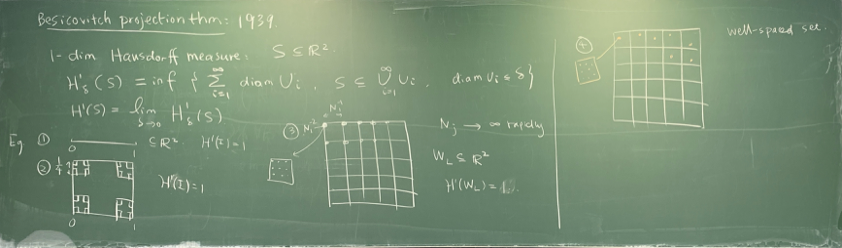
\includegraphics[width=1.0\textwidth]{images/img_20250430_151218}
  \end{figure}
\end{example}

\begin{definition}
  A set $E \subseteq \mathbb{R}^2$ is \emph{purely $1$-unrectifiable} if for every Lipschitz map $f : \mathbb{R} \rightarrow \mathbb{R}^2$, we have $\mathcal{H}^1(E \cap f(\mathbb{R})) = 0$.
\end{definition}
In other words, we can't find a ``Lipschitz curve'' whose intersection with $E$ has positive $1$-Hausdorff measure.

\begin{theorem}[Besicovitch projection theorem]
  If $E \subseteq \mathbb{R}^2$ is purely $1$-unrectifiable and $0 < H^1(E) < \infty$, then $H^1(\pi_e(E)) = 0$ for $H^1$-almost every $e \in \mathbb{S}^1$, where $\pi_e : \mathbb{R}^2 \rightarrow \mathbb{R}$ is given by as $x \mapsto x \cdot e$.
\end{theorem}
Naive thoughts: if a ``quantitative Besicovitch projection theorem'' is true, then for most of the $\eps$-separated directions $e$, we have that $\pi_{\ell}(W)$ is small.  This shows that the $\eps$-net version of the set does not exist.  But this turns out to be too wishful thinking -- it's not true, as we'll explain for the rest of the talk.

The \textbf{difficulty} is that at scale $\eps = N_1^{- 2}$, it's hard to distinguish well-spaced sets and a line via orthogonal projections.

As for our lattice: take $W$ to be an $\eps$-neighborhood of $ \left( \frac{1}{10 N_1} \mathbb{Z} \cap[0, 1] \right)^2.$  Let $\theta =(1, x)$.  Inductivey, write
\begin{equation*}
  \left\lvert x - \tfrac{p}{q}
  \right\rvert < \frac{1}{q_{N_1}}, \quad(p, q) = 1, \quad p \approx q \approx N_1.
\end{equation*}
This is true for $\gtrsim 1$ fraction of $x \in[0, 1]$.  Then $\pi_\theta W$ contains an interval of length $\approx 1$.  The shapes of the bad direction regions can be a couple different ones.

\begin{figure}
  \centering
  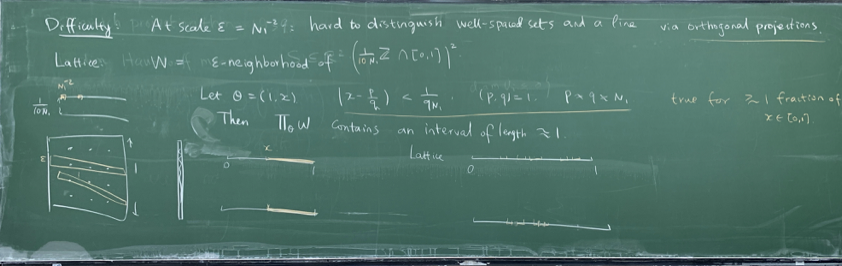
\includegraphics[width=1.0\textwidth]{images/img_20250430_153653}
\end{figure}

\section{Damaris Schindler, \emph{Density of rational points near manifolds}}

Let $M \subseteq \mathbb{R}^n$ be a manifold of dimension $m$.  Denote by $R := n - m$ the codimension.  For $Q > 1$ and $0 \leq \delta < 1/2$, let $N_M(Q, \delta)$ denote the number of rational vectors $p / q \in \mathbb{Q}^n$, with $p \in \mathbb{Z}^n$ and $1 \leq q \leq Q$, such that
\begin{equation*}
  \dist\left(M, \frac{p}{q}\right) \leq \frac{\delta}{q}.
\end{equation*}
We have the trivial bound $N_M(Q, \delta) \ll Q^{m + 1}$.  Heuristically, we expect that
\begin{equation*}
  N_M(Q, \delta) \sim Q \left( \frac{\delta}{Q} \right)^2 Q^n \sim \delta^R Q^{m + 1}.
\end{equation*}
For $\delta > 0$, we have $N_M(Q, \delta) \geq N_M(Q, 0)$.

What is the size of $N_M(Q, 0)$ for ``non-flat'' $M$?

Let $V \subseteq \mathbb{P}_Q^n$ be an irreducible variety of degree $d > 1$.  Denote by $H : \mathbb{P}_{\mathbb{Q}}^n(\mathbb{Q}) \rightarrow R_{\geq 0}$
the height function $H(\underline{x}) := \max_{0 \leq i \leq n} \lvert x_i \rvert$, for $\underline{x} =(x_0, \dotsc, x_n) \in \mathbb{Z}^{n + 1}_{\mathrm{prim}}$.  Denote by $N_V(Q)$ the number of $x \in V(\mathbb{Q})$ with $H(x) \leq Q$.
\begin{conjecture}[Weak dimension growth conjecture]
  For $d \geq 2$ and $\eps > 0$, we have $N_V(Q) \ll Q^{\dim V + \eps}$.
\end{conjecture}
\begin{example}
  Take $V = \{F = 0\}$, where $F \in \mathbb{Z}[x_0, \dotsc, x_n]$ with $\deg F \geq 2$.  Compare to $M \subseteq V \cap \{x_0 = 0\}$ given by $F(1, x_1 / x_0, \dotsc, x_n / x_0) = 0$.
\end{example}
\begin{conjecture}[Huang '20, Beresnevich--Kleinbock '22]
  If the manifold $M$ is non-flat in some sense, say it satisfies ``proper curvature conditions'', then if $\delta \geq Q^{- \frac{1}{k} + \eps}$, we have the asymptotic $N_M(Q, \delta) \sim \delta^R Q^{m + 1}$ as in the heuristic argument.
\end{conjecture}
Note that this implies that $N_M(Q, \delta) \leq Q^{m + \eps} + \delta^R Q^{m + 1}$ for all $\delta$.

This conjecture has been proved by Huang '20 for smooth hypersurfaces of non-vanishing Gaussian curvature with $m \geq 2$.  This is proved using methods purely from harmonic analysis.  It's interesting because we can also run the above argument backwards: if we have an algebraic variety that satisfies this conditions on curvature, then we can stick the affine patches of our variety into the above conjecture and then get back the dimension growth conjecture.  We get the weak dimension growth conjecture for hypersurfaces which satisfy the curvature condition.

Let's give a proof sketch.  Locally parametrize $M$ as $(\underline{x}, f_1(\underline{x}), \dotsc, f_R(\underline{x}))$, with $\underline{x} \in \mathbb{R}^m$.  Then
\begin{equation*}
  N(Q, \delta) \sim \sum_{
    \substack{
      1 \leq q \leq Q  \\
      a \in \mathbb{Z}^m
    }
  }
  \omega\Bigl(\frac{a}{q}\Bigr)
  \prod_{i = 1}^R \omega_0 \left( \frac{\lVert q f_i(\frac{a}{q}) \rVert}{\delta} \right).
\end{equation*}
This last factor effectively enforces the condition that $\lvert f_i(\tfrac{a}{q}) - \frac{b_i}{q} \rvert \leq \frac{\delta}{q}$ for some integer $b_i$.  The above should be
\begin{align*}
  &\sim \delta^R \sum_{
                                                                         \substack{
                                                                         q \leq Q  \\
  a \in \mathbb{Z}^m
  }
  } \omega \left( \frac{a}{q} \right)
  +(\mathrm{error}) \\
                                                                      &\sim \delta^R Q^{m + 1} + (\mathrm{error}).
\end{align*}
The error term here is
\begin{equation*}
  \ll \sum_{j \in \mathbb{Z}^R - \{0\}}
  b_{\delta, j}
  \sum_{
    \substack{
      q \leq Q  \\
      a \in \mathbb{Z}^m
    }
  }
  \omega \left( \frac{a}{q} \right)
  e \left( q \sum_{i = 1}^R j_i f_i \left( \frac{a}{q} \right) \right).
\end{equation*}
Here the meaningful range is $j \ll Q^\eps / \delta$.  Now, maybe you want to apply Poisson summation to the sum over $a$.  This gives
\begin{equation*}
  \sum_{q \leq Q} q^m \sum_{k \in \mathbb{Z}^m} I(q, j, k),
\end{equation*}
where
\begin{equation*}
  I(q, j, k) = \int_{\mathbb{R}^m} \omega(x) e \left( q \left( \sum_{i = 1}^R j_i f_i(x) - k \cdot x \right) \right) \, d x.
\end{equation*}
Now we stick to $R = 1$ and assume non-vanishing Gaussian curvature.  Then, if there exists a critical point $x_0 =(\nabla f)^{-1} \left( \frac{k}{j} \right)$ (there is only one index $j$ left, so we drop the index), then
\begin{equation*}
  I(q, j, k) \sim e \left( q j \left( f(x_0) - \frac{k}{j} x_0 \right) \right)(q j)^{- \frac{m}{2}}.
\end{equation*}
We define the ``dual'' or ``Legendre dual'' of $f$ to be
\begin{equation*}
  f^\ast(y) := x \cdot y - f(x) \text{ if } y = \nabla f(x).
\end{equation*}
Taking the dual of the phase of interest and summing, we obtain
\begin{equation*}
  \sum_{q \leq Q} e\left(- q j f^\ast \left( \frac{k}{j} \right)\right),
\end{equation*}
which leads us to asking for the number of $j \ll Q^\eps \delta^{-1}$ and $k \ll Q^\eps \delta^{-1}$ with $\lVert   j f^\ast ( k/j ) \rVert$ small.  We then iterate.

Frequently asked questions:
\begin{itemize}
\item Full alternative proof for dimension growth conjecture?  For example, the cone over an algebraic variety violates the curvature condition.
\item Curvature in higher codimension?
\item ``Proper curvature conditions''?  We explain below.
\end{itemize}
\begin{definition}
  Let $M \subseteq \mathbb{R}^n$ be given locally by $(x, f_1(x), \dotsc, f_R(x))$, again with $x \in \mathbb{R}^m$.  Then we say that $M$ is $\ell$\emph{-non-degenerate at $x_0 \in \mathbb{R}^m$} if all the partitions derivatives in $x$ of order up to $\ell$ of $(x, f_1(x), \dotsc, f_R(x))$ span $\mathbb{R}^n$.
\end{definition}
\begin{example}
  If $R = 1$ and you have a hypersurface, then to be $\ell$-non-degenerate, there should be a partial derivative of order up to $\ell$ that is nonvanishing.
\end{example}
\begin{conjecture}[Huang '22]
  If $M$ is $(R + 1)$-non-degenerate and $\delta \geq Q^{- \frac{1}{R} + \eps}$, then we expect the heuristic asymptotic $N_M(Q, \delta) \sim \delta^R Q^{m + 1}$ to hold.
\end{conjecture}
(Consider $(x_1, \dotsc, x_m, x_1^{\ell}, \dotsc, x_R^{\ell})$.)


\section{Trevor Wooley, \emph{The paucity of knowledge concerning Weyl sums and their mean values}}

\subsection{Introduction}

Consider a Vinogradov exponential sum
\begin{equation*}
  f(\alpha) := \sum_{1 \leq x \leq N} e(\alpha_1 x + \dotsb + \alpha_k x^k).
\end{equation*}
Here $N$ is a large positive integer, $e(z) := e^{2 \pi i z}$.  We will specialize to the case $k = 1$:
\begin{equation*}
  f(\alpha) = \sum_{1 \leq x \leq N} e(\alpha x^k).
\end{equation*}
(Circle method) complexity of $\alpha$:
\begin{equation*}
  H(\alpha) :=
  H(\alpha; N^k)
  =
  \min_{
    \substack{
      a \in \mathbb{Z}  \\
      q \in \mathbb{N}
    }
  }
  \left\{ q + N^k \lvert q \alpha - a \rvert \right\}.
\end{equation*}
Informally, this will be small if $\alpha$ has good rational approximations.

Dirichlet: given $\alpha \in \mathbb{R}$, there exists $a \in \mathbb{Z}$, $q \in \mathbb{N}$ with $1 \leq q \leq N^{k/2}$ and $\lvert q \alpha - a \rvert \leq N^{- k/2}$ such that
\begin{equation*}
  H(\alpha) \leq q + N^k \lvert q \alpha - a \rvert \leq 2 N^{k/2}.
\end{equation*}
Thus, if $H(\alpha) = Q$, then there exists $a \in \mathbb{Z}$, $q \in \mathbb{N}$ with $(a, q) = 1$ such that $q \leq Q$ and $\lvert q \alpha - a \rvert \leq Q N^{- k}$.

One basic question in the subject is to understand the behavior of an exponential sum like $f(\alpha)$ for $1 \leq H(\alpha) \leq 2 N^{k/2}$.  Three trivial ranges for $H(\alpha)$:

\textbf{Range (0).}
$H(\alpha) \ll 1$.  Say $\left\lvert \alpha - \tfrac{a}{q} \right\rvert \leq \frac{1}{100} N^{- k}$, where $q \leq 100$.  Then $\lvert f(\alpha) \rvert \approx N$.

\textbf{Range (1).}
$H(\alpha) \ll N$.  Use mean value theorem.  We have $\alpha = \beta + a/q$, say.  Then
\begin{align*}
  f(\alpha)
  &= \sum_{1 \leq x \leq N} e \left((\beta + a/q) x^k \right)
                                                                                                    =
                                                                                                    \sum_{r = 1}^q \sum_{
                                                                                                    \substack{
                                                                                                    \frac{1 - r}{q} \leq y \leq \frac{N - r}{q}  \\
  x = q y + r
  }
  }
  e \left((\beta + \tfrac{a}{q})(q y + r)^k \right) \\
                                                                                                 &=
                                                                                                    \sum_{r = 1}^q e \left( \frac{a}{q} r^k \right)
                                                                                                    \sum_{\frac{1 - r}{q} \leq y \leq \frac{N - r}{q}}
                                                                                                    e \left( \beta(q y + r)^k \right) \\
                                                                                                 &=
                                                                                                    \sum_{r = 1}^q e  \left( \frac{a}{q} r^k \right) \left( q^{-1} \int_0^N e(\beta \gamma^k) \, d \gamma
                                                                                                    + \O\left(1 + N^k \lvert \beta \rvert\right)\right) \\
                                                                                                 &=q^{-1} S(q, a) v(\beta) + \O \underbrace
                                                                                                    {
                                                                                                    \left( q + N^k \lvert q \alpha - a \rvert  \right)
                                                                                                    }_{
                                                                                                    H(\alpha)
                                                                                                    },
\end{align*}
where
\begin{equation*}
  S(q, a) := \sum_{r = 1}^q e \left( \frac{a}{q} r^k \right),
  \quad
  v(\beta) = \int_0^N e(\beta \gamma h) \, d \gamma.
\end{equation*}
Vaughan, 1981: use Poisson summation to refine this estimate, giving
\begin{equation*}
  f(\alpha) - q^{-1} S(q, a) v(\beta) \ll H(\alpha)^{1/2 + \eps}.
\end{equation*}

Note: this gives
\begin{equation*}
  f(\alpha) - q^{-1} S(q, a) v(\beta) \ll N^{k/4 + \eps},
\end{equation*}
but if $k \geq 4$, then this is worse than trivial.  That's bad news, but what it does show is that at last when $H(\alpha) \leq N$, the error term is $\O(N^{1/2 + \eps})$.  This gives
\begin{equation*}
  \int_{H(\alpha) \leq N} \lvert f(\alpha) \rvert^s \, d \alpha \ll N^{s - k + \eps}
  \quad
  \text{when }
  \begin{cases}
    s \geq k + 1
    & \text{ if } k \geq 3, \\
    s \geq k + 2
                                                                                            & \text{ if } k = 2.
  \end{cases}
\end{equation*}

We should mention that Vaughan, 1981, had what he would like to call a ``speculation'' (not a conjecture): that
\begin{equation*}
  f(\alpha) - q^{-1} S(q, a) v(\beta) \ll H(\alpha)^{1/k + \eps}.
\end{equation*}
Remember that $H(\alpha)$ can be as large as $N^{k/2}$, so this is $\sqrt{N}$ in the worst case, but usually much better.  However, this speculation was shown to be false in work of Brüdern--Daemen
published in 2009.  There is much more that was proved in this work, but in particular,
\begin{equation*}
  \lvert f(\alpha) - q^{-1} S(q, a) v(\beta) \rvert \gg N^{1/2}
\end{equation*}
for almost all $\alpha$.

\begin{conjecture}
  We have $f(\alpha) - q^{-1} S(q, a) v(\beta) \ll N^{1/2 + \eps}$ for $H(\alpha) \leq 2 N^{k/2}$.
\end{conjecture}

\begin{problem}[Challenge Problem]
  Take $k$ large, $q \approx N^3$.  Estimate
  \begin{equation*}
    \left\lvert \sum_{1 \leq x \leq N} e \left( \frac{a}{q} x^k \right)
      - \frac{N}{q}
      S(q, a)\right\rvert
    \ll N^\theta,
  \end{equation*}
  where
  \begin{equation*}
    \theta < \min \left\{ \frac{k}{4}, \theta_0 \right\},
  \end{equation*}
  with $\theta_0$ independent of $k$ and $< 1$.
\end{problem}

\subsection{How little we know}

Let's focus on
\begin{equation*}
  f\left(\frac{a}{q}\right) = \sum_{1 \leq x \leq N}
  e \left( \frac{a}{q} x^k \right).
\end{equation*}
The usual approach:

\textbf{(A) Weyl's inequality}.  Write
\begin{equation*}
  \lvert f(\alpha) \rvert^2 = f(\alpha) f(- \alpha)
  = \sum_h \sum_x e \left( \alpha \left((x + h)^k - x^k \right) \right)
  h(k x^{k - 1} + \dotsb).
\end{equation*}
This gives
\begin{equation*}
  \lvert f(\alpha) \rvert^{2^{k - 1}}
  \ll N^{2^{k - 1} - 1} + N^{2^{k - 1} - k}
  \left\lvert
    \sum_{\lvert h_1 \rvert \leq N} \dotsb \sum_{
      \substack{
        \left\lvert h_{k-1}\right\rvert \leq N   \\
        h_1 \dotsb h_{k - 1 \neq 0}
      }
    }
    e \left( h_1 \dotsb h_{k - 1} \alpha(k ! x + c(h)) \right)
  \right\rvert,
\end{equation*}
giving
\begin{align*}
  f\left(\frac{a}{q}\right)
  &\ll N^{2^{k - 1} - 1} + N^{2^{k - 1} - k + \eps}
  \sum_{1 \leq h \leq k ! N^{k - 1}} \min \left\{ N, \left\lVert h \frac{a}{q} \right\rVert^{-1} \right\} \\
  &\ll \left(N^{1 + \eps}
    \left( q^{-1} + N^{-1} + q N^{- k} \right)^{2^{1 - k}} \right)^{2^{k - 1}}.
\end{align*}

\textbf{(B) Vinogradov, I.}  There's various ways of setting up this approach, which more-or-less amount to the same thing.  We'll choose the one that is easiest to describe from first principles.  It is slightly wasteful, but illustrates the right ideas.
\begin{equation*}
  \left\lvert f(\alpha) \right\rvert^2 = \sum_{\lvert h \rvert \leq N}
  \sum_{x \in I(h)} e \left( h \alpha(k x^{k - 1} + \dotsb) \right).
\end{equation*}
Then
\begin{align*}
  \left\lvert f(\alpha) \right\rvert^{4 s}
  &\leq N^{2 s - 1} \sum_{\lvert h \rvert \leq N}
  \left\lvert
    \sum_{x \in I(h)}
    e \left( h \alpha(k x^{k - 1} + \dotsb) \right)
    \right\rvert^{2 s} \\
  &\leq N^{2 s - 1} \sum_{\lvert h \rvert \leq N}
    \left\lvert
    \sum_{x_1, \dotsc, x_{2 s}}
    e \left( h \alpha(k v_{k - 1}(x) + \dotsb) \right)
    \right\rvert, \\
\end{align*}
where $\sigma_j(x) = x_1^j + \dotsb + x_s^j - x_{s + 1}^j - \dotsb - x_{2 s}^j$.  Write $\sigma_j(x) = \ell_j$ for $1 \leq j \leq k - 1$.  Then by fixing the values of the $\ell_j$ and counting, we obtain
\begin{equation*}
  \lvert f(\alpha) \rvert^{4 s} \leq N^{2 s - 1}
  \cdot N^{1 + 2 + \dotsb +(k - 2)}
  J_{s, k - 1}(N) \cdot \left\lvert \sum_{\lvert h \rvert \leq N} \sum_{\lvert \ell \rvert \leq s N^{k - 1}}
    e \left( k h \ell \alpha \right)\right\rvert,
\end{equation*}
where
\begin{align*}
  J_{s, k - 1}(N)
  &= \# \left\{ \sum_{i = 1}^s
    (x_i^j - y_i^j) = 0 \quad (1 \leq j \leq k - 1) \, : \, 1 \leq x, y \leq N \right\} \\
  &\ll
    N^{2 s - \tfrac{1}{2} k(k - 1) + \eps}
    + N^{s + \eps}.
\end{align*}
(Bourgain--Demeter--Guth, 2016, Wooley, 2016/2019.)  Glueing together all of these estimates, we get an upper bound
\begin{equation*}
  \left\lvert f \left( \frac{a}{q} \right) \right\rvert \ll N^{1 + \eps} \left( \frac{1}{q} + N^{-1} + q N^{- k} \right)^{1/k(k - 1)}.
\end{equation*}

\textbf{(C) Vinogradov, II (Bombieri--Korobov).}  Replace the initial exponential sum with shifts:
\begin{equation*}
  f(\alpha) =
  \frac{1}{U V}
  \sum_{
    \substack{
      u \sim U  \\
      v \sim V
    }
  }
  \sum_{1 \leq x \leq N} e \left( \alpha(x + u v)^k \right).
\end{equation*}
One uses that
\begin{equation*}
  f \left( \frac{a}{q} \right)
  \ll N^{1 + \eps} \left( q^{-1} + U^{- k} + V^{- k} + q(U V)^{- k} \right)^{1/4 s^2}
\end{equation*}
for $s \geq \tfrac{1}{2} k(k + 1)$.

\subsection{Mean values}

If you can't achieve pointwise bounds, maybe you'll have more success with mean values.  The nice thing about mean values is that there are nice arithmetic interpretations for what happens.  To illustrate the ideas, we'll again look at the same exponential sum $f(\alpha)$.  We consider the integral
\begin{equation*}
  I_s(N) :=
  \int_0^1 \left\lvert f(\alpha) \right\rvert^{2 s} \, d \alpha,
\end{equation*}
which by orthogonality is counting the number of solutions to the equation
\begin{equation*}
  x_1^k + \dotsb + x_s^k = x_{s + 1}^k + \dotsb + x_{2 s}^k \quad(1 \leq x_i \leq  N).
\end{equation*}
We conjecture that
\begin{equation*}
  I_s(N) \sim \left( C N^{2 s - k} + s ! N^s \right)(1 + o(1)).
\end{equation*}
Here $C$ is a product of local densities, $H(\alpha) \leq N$, and the second term comes from the diagonal solutions where $\{x_1, \dotsc, x_s\} = \{x_{s + 1}, \dotsc, x_{2 s}\}$.

The basic question for these mean values from the point of view of the circle method is to understand the source of the various contributions to this mean value $I_s(N)$ arising from points $\alpha$ in the full range $1 \leq H(\alpha) \leq 2 N^{k/2}$.

As a challenge, identify the source of the diagonal solutions (arising from linear spaces).  The contribution from the small height is
\begin{equation*}
  \int_{H(\alpha) \leq N} \left\lvert f(\alpha) \right\rvert^{2 s} \sim C N^{2 s - k},
\end{equation*}
where $C$ is a product of local densities.
\begin{conjecture}[Vaughan and Wooley, 1995]
  \begin{equation*}
    \int_{N < H(\alpha) \leq 2 N^{k/2}}
    \left\lvert f(\alpha) \right\rvert^{2 s} \, d \alpha \sim \text{contribution of special subvarieties}.
  \end{equation*}
\end{conjecture}
\begin{example}
  We were able to show that
  \begin{equation*}
    \int_0^1 \int_0^1 \left\lvert \sum_{1 \leq x \leq N} e(a x^3 + \beta x) \right\rvert^6
    \, d \alpha \, d \beta = 6 N^3 + C N^2(\log N)^5(1 + o(1)).
  \end{equation*}
  (``$C$'' is due to de la Breteche.)
\end{example}
\begin{example}[Brüdern--Wooley, 2019]
  \begin{equation*}
    \int_{[0, 1]^3} \left\lvert \sum_{\lvert x \rvert \leq N} e(\alpha x^3 + \beta x) \right\rvert^6
    \left\lvert \sum_{\lvert x \rvert \leq N} e(\alpha x^3 + \gamma x) \right\rvert^4
    \, d \alpha \, d \beta \, d \gamma
    \sim
    (45 + \mathcal{C}) N^3(1 + o(1)).
  \end{equation*}
  Here $\mathcal{C}$ is again a product of local densities.
\end{example}
\begin{example}
  \begin{align*}
    \int_0^1 \left\lvert \sum_{1 \leq x \leq N}
    e(\alpha x^4)\right\rvert^6 \, d \alpha
    &=
      \# \left\{ x_1^4 + x_2^4 + x_3^4 = x_4^4 + x_5^4 + x_6^4 : 1 \leq x_i \leq N \right\} \\
    &\sim 3! N^3 + \mathcal{C} N^2
      + \mathcal{C} ' N^2 \log N.
  \end{align*}
  Here
  \begin{itemize}
  \item the first term comes from the diagonal,
  \item in the second term, $\mathcal{C}$ is a product of local densities, and we have $H(\alpha) \leq N$, and
  \item the third term comes from the contribution of
    \begin{align*}
      x_3 &= x_1 + x_2, \\
      x_6 &= x_4 + x_5, \\
      x_1^2 + x_1 x_2 + x_2^2 &= x_4^2 + x_4 x_5 + x_5^2.
    \end{align*}
    This uses the identity $a^4 + b^4 +(a + b)^4 = 2(a^2 + a b + b^2)^2$.
  \end{itemize}
\end{example}

Let's now describe a \textbf{model problem} to think about, which embodies many of the characteristics we see here and gets back to the observation about pointwise estimates boiling down to understand congruences and glueing variables to make the summation length bigger than the congruence modulus.  The model problem is to obtain ``good'' estimates for the $q$-analogue problem, by which we mean
\begin{equation*}
  \left\{ x_1^k + \dotsb + x_s^k \equiv x_{s + 1}^k + \dotsb + x_{2 s}^k \pmod{q},
    \,
    1 \leq x_i \leq N\right\}
  = \frac{1}{q}
  \sum_{a = 1}^q \left\lvert f \left( \frac{a}{q} \right) \right\rvert^{2 s},
\end{equation*}
with $q$ fixed and $N^2 < q \leq N^{k / 2}$.  What's going on in this problem is that if $q \leq N$, then this problem really looks like the congruence problem, because the variables are big enough that you can just reduce things to congruences -- it's just a $\mathbb{Z} / q \mathbb{Z}$ problem.  On the other hand, for $q > N^k$, you have to consider equations.

\section{Po Lam Yung, \emph{Discrete restriction in 2+1 vs 1+1 dimensions}}
[Slide talk, notes very partial]


\begin{equation*}
  \mathcal{I}(a) := \left\lVert \sum_{n \in \mathbb{Z}} a_n e(n x + n^2 t) \right\rVert_{L^6([0, 1]^2)}.
\end{equation*}
Bourgain--Demeter: if $\supp(a) \subseteq[N]$, then
\begin{equation*}
  \mathcal{I}(a) \lesssim_\eps N^\eps \lVert a \rVert_{\ell_2}.
\end{equation*}
Discrete version of Fourier restriction for the parabola.

Bourgain: for $a$ the indicator function on $[N]$,
\begin{equation*}
  \mathcal{I}(a) \gtrsim(\log N)^{1/6} \lVert a \rVert_{\ell_2}.
\end{equation*}
Circle method shows reverse inequality is true for this $a$.

Herr--Kwak: if $a$ is supported in a finite set $E \subseteq \mathbb{Z}^2$, then
\begin{equation*}
  \left\lVert \sum_{n \in E} a_n e(n \cdot x + \lvert n \rvert^2 t) \right\rVert_{L^4([0, 1]^3)} \lesssim(\log \# E)^{1/4} \lVert a_n \rVert_{\ell_2}.
\end{equation*}
Obtaining the sharp power of log allows them to study global well-posedness for the cubic non-linear Schrödinger equation on $\mathbb{T}^2$,
\begin{equation*}
  i \partial_t u + \Delta_x u = \pm \lvert u \rvert^2 u,
\end{equation*}
which is $L^2$-critical.

We have, with $\tilde{n} :=(n, \lvert n \rvert^2)$ for $n \in \mathbb{R}^2$,
\begin{equation*}
  \int_{[0, 1]^3}
  \left\lvert \sum_{n \in E} e(n \cdot x + \lvert n \rvert^2 t) \right\rvert^4 \, d x \, d t
  = \# \left\{(n_1, n_2, n_3, n_4) \in E^4 : \tilde{n}_1 - \tilde{n}_2 = \tilde{n}_4 - \tilde{n}_3 \right\}
\end{equation*}
ist eh number of parallelograms in $\mathbb{R}^3$ with all vertices in $\tilde{E}$.

Observation: the $\tilde{n}_j$ form a parallelogram in $\mathbb{R}^3$ if and only if the $n_j$ form a rectangle in $\mathbb{R}^2$.

Pach and Sharir (1990s): the number of rectangles with vertices in $E$ is $\lesssim(\# E)^2 \log(\# E)$.
\end{document}
